\documentclass[11pt, a4paper]{article} % , draft
\usepackage[utf8]{inputenc}

\usepackage{enumitem} % customiçe item dots etc
\usepackage{textgreek} % obv
\usepackage{physics} % for easy derivative notation
\usepackage{amsmath}
\usepackage{amsthm} %theorems
\usepackage{amssymb}
\usepackage{mathtools} % for matrices with blocks inside
\usepackage[scr=boondoxo]{mathalfa}
\usepackage{pst-node}%
\usepackage{mathrsfs}
\DeclareMathAlphabet{\mathpzc}{OT1}{pzc}{m}{it}

\newcommand{\mc}{\multicolumn{1}{c}}
\newcommand{\R}{\mathbb{R}} % command for real R
\newcommand{\Holo}{\mathcal{H}}
\newcommand{\M}{\mathcal{M}}
\newcommand{\C}{\mathbb{C}}
\newcommand{\N}{\mathbb{N}}
\newcommand{\z}{\mathpzc{s}}
\newcommand{\p}{\mathpzc{r}}
\newcommand{\s}{\mathbb{S}}
\newcommand{\W}{\mathbb{W}}
\newcommand{\U}{\mathscr{U}}
\newcommand{\Lg}{\mathscr{L}}
\newcommand{\x}{\mathcal{X}}

\usepackage{csquotes}
\MakeOuterQuote{"}
\setlength{\parskip}{0.3 cm}

\usepackage{fancyhdr}

%\usepackage{nath} % authomatic parenthesis stuff
%\delimgrowth=1
\usepackage[left=2cm, right=2cm, top=2.1cm, bottom=2.1cm]{geometry} % set custom margins
\usepackage{graphicx} % to insert figures
\usepackage{grffile}
\graphicspath{{Figures/}} % define the figure folder path
\usepackage{subcaption} % for multiple figures at once each with a caption
\usepackage{multirow} %multirow in tables

\usepackage{caption}
\captionsetup[figure]{font=footnotesize} %adjust caption size
\captionsetup[table]{font=footnotesize} %adjust caption size

\usepackage{booktabs} % for pretty tabs in tables
\usepackage{siunitx} % Required for alignment
\captionsetup{labelfont=bf} % bold face captations

\usepackage{hyperref} % makes every reference a hyperlink
\hypersetup{
    colorlinks=true,
    linkcolor=violet,
    filecolor=[rgb]{0.69, 0.19, 0.38},      
    urlcolor=[rgb]{0.0, 0.81, 0.82},
    citecolor=[rgb]{0.69, 0.19, 0.38}
}

\usepackage{epigraph} % for quotations in teh begginig
\setlength\epigraphwidth{8cm}
\setlength\epigraphrule{0pt}
\usepackage{etoolbox}
\makeatletter
\patchcmd{\epigraph}{\@epitext{#1}}{\itshape\@epitext{#1}}{}{}
\renewcommand{\qedsymbol}{o.\textepsilon.\textdelta}

\newtheorem{prop}{Proposition} %so I can use propositions
\newtheorem{cor}{Corollary} %so I can use corollaries
\newtheorem{defi}{Definition} %so I can use corollaries

\makeatother % all this is for the epigraph
\usepackage{tocloft}

\usepackage{imakeidx} % make index

\makeindex[columns=3, title=Alphabetical Index, intoc]

%\title{\vspace{-2.5cm} {\bf Can we make the Exponential scaling in Time\\ be Linear in Time if Parallelized Exponentially? \\ {\em - Part 2 -}} \vspace{-0.4cm}  }
\title{\vspace{-2cm} {\bf An Intuitive Narrative for\\ Open Quantum Systems?}\\{\small by {\em Xabier Oyanguren Asua}}\vspace{-0.8cm}}
\date{\vspace{-11ex}}
\let\clipbox\relax
\usepackage{adjustbox}
\newcolumntype{?}{!{\vrule width 1.5pt}}
\usepackage{abstract}
\setlength{\absleftindent}{0mm}
\setlength{\absrightindent}{0mm}

\usepackage{tcolorbox}
\DeclareRobustCommand{\mybox}[2][gray!10]{%
\begin{tcolorbox}[   %% Adjust the following parameters at will.
        left=0.2cm,
        right=0.2cm,
        top=0.15cm,
        bottom=0.15cm,
        colback=#1,
        colframe=#1,
        width=\dimexpr\textwidth\relax, 
        enlarge left by=0mm,
        boxsep=5pt,
        arc=0pt,outer arc=0pt,
        ]
        #2
\end{tcolorbox}
}


\usepackage{anyfontsize}

\NewDocumentEnvironment{kapituloBerria}{mm}
{\clearpage           % we want a new page          %% I commented this
   \thispagestyle{empty}% no header and footer
   \vspace*{\stretch{2}}% some space at the top
   \raggedleft          % flush to the right margin
   {\textbf{{\fontsize{60}{40}\selectfont \hspace{+9.5cm}#1 \newline \newline}}}
   \bf
   \fontsize{30}{20}\selectfont
  }
  {\par % end the paragraph
   \vspace{\stretch{3}} % space at bottom is three times that at the top
   \normalfont
      \fontsize{15}{20}\selectfont
      \vspace{-1cm}
   \begin{flushleft}{ \textit{#2}  }
   \end{flushleft}
   \clearpage           % finish off the page
  }
  
%\newenvironment{kapituloBerria}[2]
  

\usepackage{listings}
\usepackage{xcolor}
\lstset{language=C++,
                basicstyle=\ttfamily,
                keywordstyle=\color{blue}\ttfamily,
                stringstyle=\color{red}\ttfamily,
                commentstyle=\color{green}\ttfamily,
                morecomment=[l][\color{magenta}]{\#}
    backgroundcolor=\color{black!5}, % set backgroundcolor
    basicstyle=\footnotesize,% basic font setting
}

\begin{document}

\clearpage
%% temporary titles
% command to provide stretchy vertical space in proportion
\newcommand\nbvspace[1][3]{\vspace*{\stretch{#1}}}
% allow some slack to avoid under/overfull boxes
\newcommand\nbstretchyspace{\spaceskip0.5em plus 0.25em minus 0.25em}
% To improve spacing on titlepages
\newcommand{\nbtitlestretch}{\spaceskip0.6em}
\pagestyle{empty}
\begin{center}
\bfseries
\nbvspace[1]
\Huge
{\nbtitlestretch\huge
AN INTUITIVE NARRATIVE FOR\\
OPEN QUANTUM SYSTEMS?
}

\nbvspace[1]
\normalsize

AN AXIOMATIC APPROACH TO \\
MAKE QUANTUM MEASUREMENTS\\ 
AND OPEN SYSTEM DYNAMICS\\ INTUITIVE \\

\nbvspace[1]

%Minimizing unjustified assumptions

\nbvspace[1]
\small BY\\
\Large Xabier Oyanguren Asua\\[0.5em]
%\footnotesize Can we really foresee the future of the Universe?"\\


\nbvspace[6]


\includegraphics[width=2.5in]{UAB.png}
\normalsize
\vspace{-0.5cm}
%\small Thesis Directors: \\
%\nbvspace[0.2]
%\large Jordi Mompart Penina \\
%Xavier Oriols Pladevall\\
%\nbvspace[1]

%Universitat Autònoma de Barcelona\\
\large
%DEGREE FINAL DISSERTATION \\
\small
%Bachelor's degree in Nanoscience and Nanotechnology \\
\small
$\ $Winter 2021-2022
\nbvspace[1]
\end{center}
\newpage
\null
\clearpage

\maketitle
\pagenumbering{gobble}
\setlength{\cftbeforesecskip}{0.4cm}
\setlength{\cftbeforesubsecskip}{0.4cm}
\setlength{\cftbeforesubsubsecskip}{0.25cm}

\tableofcontents
\clearpage
\pagenumbering{arabic}
\setcounter{page}{0}
\vspace{-0.3 cm}

\pagestyle{empty}

\section*{Abstract}


\section*{Objectives}\vspace{-0.2cm}



\section*{Guideline}\vspace{-0.2cm}


\newpage
\pagestyle{fancy}
\fancyhead[L]{Philosophical Prolegomena}
\fancyhead[R]{\em On the Noumenon and Phenomenon}

\section*{\centering \huge{Philosophical Prolegomena}} %Preface
\addcontentsline{toc}{section}{Philosophical Prolegomena}
\subsection*{On the Noumenon and Phenomenon}
\addcontentsline{toc}{subsection}{On the Noumenon and Phenomenon}

Focus your attention for a moment in that thing that is behind the eyes that are reading these lines and in front of the back of your head. Perhaps a bit upper than the eyes. There, in the center of your "world" or reality. We call it {\bf consciousness}. It is you, the light that makes you. That thing that when a person expels the last breath, is no longer there \footnote{It is no longer there when you are deep asleep either...}. That thing that when you look at the eyes of another person, you are (or at least expect to be) looking at. The relevance of that thing, the self-aware consciousness, is the following. Imagine you discover that the reality you considered as true and contingent and objectively material, is actually fake. For example, that your brain is actually in a liquid tank in some lab and it has connected to its visual-, auditive-, self-body internal perceptive- etc. cortices or brain regions, some electrodes that stimulate the exact same neural pulses that would be stimulated by a true perception in the visual neurons of a human eye that could be reading this, tactile neurons that could be wearing those clothes or internal nerves that would feel the body extension you feel. Well, there is absolutely no way to prove that this is not indeed the case. No way. Thus, there is no way either to prove that behind the eyes of the rest of the people there is a consciousness like yours. There is actually no way either to prove that your brain was not spontaneously arranged in the vacuum of space due to statistical fluctuations with these exact memories and current perceptions. Not either that it is not the product of a super-computer simulating each and every electron and fundamental particle in your brain to the quantum level, with these cortices being activated according to the algorithm of the machine, to make you feel this reality. There is no way either, in this line, to know that this consciousness should have any sort of ontologically material cause or foundation. \vspace{-0.3cm}

So yeah, everything could simply be "fake". Well, everything, except for one thing: that {\em you}, that light of self-awareness that is behind those eyes, that, which we call {\em you}, exists. The fact that {\em you} exist is necessarily true for you. It needs no prove, because from the moment in which you are able to think, its existence is a necessity. Pause and ponder it for a moment, and realize about its trueness. We are not talking about the rest of humanity, just you, in your awareness. The rest of humans could also be fake together with the perceptual reality you are placed in. But as long as you "think", you are: you exist. No possible discussion about it. {\em "Cogito ergo sum"}, I think, therefore I am, Descartes' famous statement.

Great, so now we are both on the same beginning of the story. Let us call that "self-aware-conscious-light" that is currently reading this, simply as "the {\em cogito}".

Now, lets make explicit the first assumption or postulate that any human being makes everyday: there exists an objective and materially contingent external reality, in which your {\em cogito} is placed as a cursor in a stage. Your {\em cogito} doesn't know directly about this scenario, else the stage itself would be part of the same mind. Instead, your {\em cogito} is attached to some organic sensors, like the neurons in your eardrum, which get activated in different ways according to how the external reality modulates the shape of the eardrum membrane. Accordingly it generates a signal that the neurons send to the acoustic cortex or region in your brain. The same happens for some visual neurons that are excited in different ways as a function of the energy of the light arriving to them etc. The same for the olfactory, gustatory, tactile, accelerometric (the inner ear liquid that lets you know the direction of gravity) or proprioceptive nerves\footnote{Proprioception is the information we receive from muscles, tendons and joints that allow us to know where our body parts are at any given moment even if we close our eyes.}. Once all this information arrives to the brain, it is processed and each chunk is projected as perceptual feelings surrounding the center of your person, around your {\em cogito}. As such, the particular colors, tastes, sounds etc, you will feel are generated in that processing, presumably due to specific excitations in the sensor organs\footnote{Think about how unique those projections you feel are, that you will never be able to know if what you "see" and call "red" is not seen by another person as what you call "blue", just that you both agree it is called "red".}. Let us give these concepts some names: the "external" reality to your {\em cogito}, the reality "in itself", the one you will never know about, because you can only know through your perceptual sensors, is called {\em \bf noumenon} (assuming of course, that such a thing objectively exists with the same certainty as your own {\em cogito}). Meanwhile, the set of projections where your {\em cogito} is centered, all that "virtual" surrounding that the processing of your perceptions produces around your {\em cogito}, is called the {\em \bf phenomenon}. Of course, it is also convenient to accept the hypothesis that not only there is an objective {\em noumenon}, but that the rest of people have also behind those eyes, their own {\em cogito}, and that those {\em cogito}-s are also centered at a {\em phenomenon}, which is at least very similar to yours.

Now, note that what you know about the "external" reality is necessarily restricted to the particular way in which it is projected in your {\em phenomenon}! That is, about this {\em noumeno}, you will never know anything that cannot be directly or indirectly sensed and represented into your phenomenon. We are imprisoned in our phenomena. To convince you even more about the tangential nature of the {\em phenomenon} and {\em noumenon}, let me remember you that whenever you are dreaming, you see and touch things or even feel your own body in configurations, that are really "not true". Your brain is generating directly in the visual, auditive and other cortices, the same neuronal excitations that would be generated if your eyes received that light, or your arms were in that disposition, when in reality your eyes are closed and your arms are still hugging your teddy bear. So yeah, dreaming is indeed the most immersive of the virtual realities. If you had a computer stimulating those regions with those same pulses, you would feel the same projections in the phenomenon. Dreaming just has the little inconvenience that the reasoning cortex is at least partially inhibited (together with the motor cortex -the one making your body actually move). That is why you feel more "instinctive" and less aware, like if your judgment was covered in a sort of veil. That is why you never confuse the oneiric- with the daylight- phenomenon. Clearly, if you made the inhuman experiment to avoid the rational cortex to be inhibited, you would entirely feel a dream, as real as right now, following the fact that if you avoid the inhibition of the motor cortex you will move in the reality as you are moving in the dream. Of course, "the plot"  of that reality would be certainly confusing and inconsistent, like for Alice was the Wonderland, but the pehnomenon in itself would feel material. Think about it.\vspace{0.3cm}

\mybox{ {\bf Extra Thoughts: Solipsism, Antropocentrism and a Cosmic Logos \\ \centerline{-The Arithmetic Paradox-} \vspace{-0.2cm}  \\ }
All this can easily lead you to {\em solipsism}, the philosophical posture where {\em you} are the only existing one, and as such, the reason of existence for all of your perceptions is your own existence. That is, {\em esse est percipi}, or whatever that {\em is}, can only {\em be}, if and while it is perceived by your {\em cogito}. That is, the Universe is as long as, or where, your {\em cogito}'s light illuminates it. That is, the Universe does not manifest its existence by itself. Instead, its "real"-ity is only as long as your {\em cogito} lights it. But sure, if you have accepted the postulate that there is such a thing as a {\em noumenon} (which you provide with existence through your phenomenon), why not accept also that there are more {\em cogito}-s lighting more {\em noumena}?\vspace{-0.2cm}  \\

At this step, you may realize that there is apparently a common {\em noumenon} for all of those {\em cogito}-s, because, the rest of {\em cogito}-s seem to report changes in their phenomena that are identifiable with changes in your own phenomeon. It is this inter-personal agreement of coherence why we know dreams are not reality. Dreams do not alter this "common" {\em noumenon}. Only {\em you} feel the oneiric phenomenon. Schrödinger tries to manifest this dilemma in his {\em Mind and Matter} with the name "Arithmetic Paradox": How can there be multiple cogito-s, each giving existence with its light to the representations projected in each individual phenomenon, but even so, exist a single and shared {\em noumenon}?\vspace{-0.2cm} \\

Realize how the problem of this reality that requires to be part of a {\em phenomenon} for its existence to be manifested, but where not all the Universe is perceived by somebody at all times, could be solved by a rather simple idea.}

\mybox{ The existence in itself of the Universe could be guaranteed without the need of having us, mammals, so casual results of evolution, which could have simply never come to live, by imagining a cosmic {\em cogito} that makes everything be explicitly manifested at all times. A {\em cogito} projecting the phenomenon of all the Universe at all times, and thus alleviating our fear of our Universe being a void theater if we were not here. We could identify this cosmic {\em cogito} with the pre-established harmony of Leibniz, perhaps a justified pretext for a greater existence or perhaps just the master algorithm that connects the perceptions that the computer simulating our brains needs to take care of. On this last idea, note that if we wanted to simulate a bunch of human brains -assuming a {\em cogito} can really emerge from non-organic computations- and make them believe they are "real" we would only need to simulate the atoms of their brains and the neural pulses generating their phenomenon, with the boundary condition of letting the different phenomenons influence each other. No need to simulate the whole Universe to make them believe they are true. \vspace{-0.2cm} \\

Notice however, before sanctifying the cosmic {\em cogito}, mother algorithm or pre-established harmony, that its existence is just one possible exit for the {\em impasse} of the arithmetic paradox over solipsism. We should never forget that the first lesson is ones {\em cogito} and that all the rest of concepts are based on postulates that build up one after the other over ones {\em cogito}. If suddenly a postulate of these erases the need of having the {\em "cogito ergo sum"} as basis for the existence, then that is cheating the argumentation. Beneath this hypothesis, there will always be the one and only undeniable true that needs no prove: {\em you exist}. Yeah, perhaps it is too anthropocentric. But it seems to be the least arbitrary and least unjustified conviction a human being could have.
}

Then, just realize that how {\em we} perceive sound or images or any other perception, is due exclusively to how our human brains process the information and manifest their corresponding projections on the phenomenon. That is, if there could be other {\em cogito}-s, evolved in different circumstances, they could have a different phenomenon to ours in front of the same stimuli or same {\em noumenon}. As an example, we know that dogs for instance, have a smaller variety of visual sensor neurons and thus end up having a phenomenon with a bi-chromatic range (they "see" in gray-scales). Now, let us call the rules that make us manifest the projections in the particular ways we do (or dogs do) as mental {\em \bf categories}. These include two kinds: the purely perceptual ones -the axioms of raw perception- and the cognitive ones -the axioms of abstraction and comprehension-. 

The \textbf{perceptual categories} are those that map, for instance, certain light energies to certain colors, certain frequencies of air oscillations to certain perceived sounds or certain kinds of molecules to certain smells. If one was to explain to a non-human intelligence what music is, would need to resort to these.

Then, there are the \textbf{cognitive categories}, that are the basic essences through which we think and understand things (and through which we are doomed to understand them, as certainly as we are doomed to undeniably feel our own existence). For example, the idea of "unity" (of "one") as a concept, of "existence", or even "boundedness", which might be derived from having the idea of "unity" and "non existence" at the same time. These at the same time imply the category of "fragmentation": the reason why when you look at a scene you are able (and doomed to do so) of seeing and understanding individually delimited and separated things, as if they had independent existence from each other. You do not see everything as a single continuum, even if in the noumenon it could be that it is so. As a taste of how the nomenon could in fact be incompatible with the "fragmentation", notice that "physics" is essentially the study of the best model about the {\em noumenon} we can build, the best story to explain and predict the behavior of the {\em noumenon} and its consequences in the phenomenon. If our current models are good enough representations of the noumenon, then we know that in reality matter is a continuum of atoms that make really no distinction of whether they belong to a chair, to this paper or your own body, meaning that our "fragmentation" category is just the way we understand things, not something fundamental about reality. Most importantly however, these cognitive axioms are in essence, where mathematics are rooted on, the axioms that build them.

\subsection*{On Models, Interpretations and Narratives}
\fancyhead[R]{\em On Models, Interpretations and Narratives }
\addcontentsline{toc}{subsection}{On Models, Interpretations and Narratives}
\begin{flushright} \em "Being able to predict reality, does not make you understand it."
\end{flushright}

We can define a {\bf physical model} or {\bf theory}, as a mathematical construction that allows the prediction of reality (that is, of the events happening on the phenomenon).

A physical model must have two elements. One is a {\bf mathematical model}, which is a self-consistent mathematical construction. The other one is a {\bf basic interpretation} of the mathematical model, which can be defined as a set of links established between the mathematical entities of the model with phenomenological qualities that appear in our perceptions.

Now, such a physical model or theory, is enough from an operational point of view. It is enough for predicting the events we can perceive, which from an utilitarian view, is all physics should be about. However, we humans, have a natural tendency towards not only building physical models, as utilitarian mathematical tools, but for also seeking semantical or narrative models about reality. Stories that can aid us conceptually and intuitively understand what could be happening in the noumenon for the model to correctly predict the events we find in the phenomenon. We can define an {\bf interpretation} or {\bf narrative} of a physical model, as a self-consistent semantic story given to the mathematical structures and elements of the theory, that go beyond the set of concepts anchored to the phenomenon by the basic interpretation we defined earlier. That is, it is a conceptual representation of the noumenon, beyond the phenomenon. A conceptual representation that is consistent with each mathematical step given in the base physical model. 

The fact that physical models or theories only speak about phenomoenological events, qualities we immediately perceive, make them falsifiable. If a certain model fails in some prediction, the model will be false for a general case. However, interpretations or narratives talk about the noumenon, which by definition is "the external reality in itself, without us perceiving it through our senses and categories". This noumenon thus can never be known in itself, it is epistemologically inaccessible. Therefore, as long as a narrative is consistent with the mathematics of the model, it will be unfalsifiable as a model for the noumenon. This is, as long as the physical model it is grounded on is not proven to be incorrect.

It is this why one could say that working on an interpretation for a physical theory is a useless task. And it is indeed, from a purely productive or utilitarian point of view. However, since being able to predict reality does not make you understand it, there is place for scientists working on narratives. Intuitively understanding a theory, does not only allow a person to better make the questions about the model that can pull it to its limits, but it is also a way to better make it understand it, remember it and use it. Just as learning a text as part of a song makes it easier to digest it, or a moral is simpler to take when first known about through a tale, so is the case for a physical theory with a simple narrative, rather than the naked basic interpretation. It is a task that might not be as creative as creating the physical model itself, but is at least as imaginative and coloring for the community that reaches it. We could compare the physical theory with the outline of a picture, which has to be created "out of nothing", and thus has a big creative merit, while we could compare the interpretation or narrative with the coloring of the outlined picture. The painter is not "creating nothing usefully new", but, it gives body, consistency, appeal and digestibility to the overall picture.

In the present dissertation an illustrative narrative for the physical model comprehended under the name "Non-Relativistic Quantum Mechanics" will be exposed, as a means of introducing an intuitive explanation of the so called Open Quantum systems and their quandary.




\newpage


\begin{kapituloBerria}{Part A}{" Quantum Mechanics is Ontologically\\ Deterministic but Epistemologically Stochastic."}
The Axioms 
\end{kapituloBerria}
\newpage
\fancyhead[L]{\null}
\fancyhead[R]{\null}
\null
\clearpage


\section*{\centering \huge{Part A: The Axioms}\vspace{-0.3cm}}
\noindent\rule{\textwidth}{0.4pt}

{\bf Axioms} or {\bf postulates}\footnote{Historically, while the word  "postulate" has had an "arbitrary supposition" connotation, the word "axiom" has had a more fundamental status, as a self-evident statement that "must" be true by its own virtue. In this work, as is done today in most texts, we will use them interchangeably since the postulates we will state to build quantum mechanics, are arbitrary decisions we will make (even if grounded in intuition), but at the same time, most will be assumptions that must be taken for the theory to hold.  } are the principles or assumptions from which the understanding of something is built up. They are principles that are rather unprovable or self-evident and are admitted as the first facts in the deductive creation of a conceptual framework. This means that if one keeps on asking $why?$ within a certain framework, the last answers one can arrive to are these axioms over which all the rest is formulated. \vspace{0.2cm}

\mybox{As an example, the following ones are some of the main axioms or postulates of physics:\vspace{-0.1cm}
\begin{itemize}
\item The postulate that the {\em noumenon}, or at least its consequences in our {\em phenomenon}, are understandable for human cognition.\footnote{Note how this is a rather arbitrary assumption (as most axioms are). The inner workings of reality could have also been incomprehensible for human cognition! Yet, till date it looks like the Universe is understandable. } 

\item The postulate that this understandability, these rational models, can be formalized mathematically as a particular example of some mathematical construction, building what we called in the preface, a physical model or theory.

\item The postulates that fix the degrees of freedom of these physical models to fit our phenomenologic observations. These are postulates about some direct or indirect experimental observations we find in the phenomenon: for example, the Planck constant is this particular number because we see/measure it to be so, or time is absolute or not because we experimentally see so etc.\vspace{-0.1cm}
\end{itemize}

It is interesting to note that in maths on the other hand, the most fundamental axioms are the {\em cognitive categories} we talked about in the prologue: unity, fragmentation, inclusion, boundedness etc. The mental categories that shape our mind. Even if it is true that over them, we then also build axioms to ground mathematical theories that may be more "arbitrary". Most importantly, note that there are no experimental postulates in mathematics. This is the reason why mathematics needs no experimental proof, and no matter how complicated a mathematical theory is, once one understands the formal proof, its trueness is obvious and self-evident. This is because in its last resort, a mathematical statement is built on fundamental concepts with which you are doomed to understand the Universe (the cognitive categories). You are inevitably tied to those concepts as well as you are tied to your own existence by the {\em cogito ergo sum}.}

Much in the same way, a narrative of a physical model, also has axioms or basic assumptions. Even if in general these are not explicited, it is a very interesting point to begin from, since these are the loose ends of the interpretation. 

In this first part of the document, we will delve with the basic postulates of the narrative that will be employed in the rest of the work. Along with the narrative concepts, we will also expose the basic mathematical structures representing them in the (non-relativistic) Quantum Theory. Thus, in this first part, we will cover most of the loose-ends of both the Quantum Theory and the present narrative.
\newpage

\fancyhead[L]{The Axioms}

\fancyhead[R]{\em The State of the Universe}
\section*{A.1. The State of the Universe}\vspace{-0.2cm}
\addcontentsline{toc}{section}{Part A: The Axioms}
\addcontentsline{toc}{subsection}{1. The State of the Universe}
% Azaldu configuration space y el fluido multiversal etc como lo hacía en el otro tratado

\subsection*{A.1.1. Reviving Postulates of Classical Mechanics}\vspace{-0.2cm}
\addcontentsline{toc}{subsubsection}{1.1. Reviving Postulates of Classical Mechanics}

If we are to provide an intuitive {\bf narrative} for a general physical model, in line with the preface, it seems reasonable that we should choose an entity we can actually observe or measure in our phenomenon as the basic quantity that can be known about. That is, the epistemological\footnote{Epistemology is the metaphysical study of what is knowable, of knowledge and know-ability.} basis of the interpretation should be a Kantian phenomenological property we perceive. In the preface, we have defined as real, the set of observations of the phenomenon that all average humans agree on. The position of the objects in the physical three dimensional space is one such property we can have an agreement on. Phenomenologically, we find that there are three orthogonal degrees of freedom in which each object can be displaced. Thus, we could define an absolute orthogonal coordinate system $\R^3$ as a scenario, where all objects extend in a fixed range of space. This picture will be dynamical, meaning that it will have the option to be different at each point of a privileged degree of freedom we will call time, defined as a Universal absolute time-line denoted by $t$. At a given time, the range of space occupied by a certain object is what we will call its {\bf position}. Following the fact that when we observe the smallest objects of reality, they all seem to be point-like, infinitesimal in spatial extension, instead of occupying a continuous range in space, we will postulate that all the objects of the Universe can be described in their last resort as cumulations of smaller objects that occupy only a single point in physical space. We will call them {\bf particles} or fragments. Assuming there are $n$ (arbitrary countable) particles in the Universe, we can model their position by stating the three numbers in the coordinate system of physical space that they occupy. As such, we could define the position of all the particles of the Universe, by specifying all these triplets. This means that the Universe as a whole has $3n=N$ {\bf degrees of freedom}, which we can set together in a same tuple $\vec{x}=(x_1,...,x_N)\in \R^N$. Each possible point $\vec{x}$ in $\R^N$ will then represent a possible configuration of the Universe. A possible arrangement of particles. It is this why we call this space, the {\bf configuration space} of the Universe. Some configurations might not be realizable at every times, so we will restrict the configuration space to a subset $\Omega_t\subseteq \R^N$. Then, we let our Universe to have an evolving configuration in time, $\vec{x}(t)$, which we will call the {\bf trajectory} of the Universe.

The reason why we said the position was an easy perceptive quality to set in common was because it is a binary property of a particle per each point in space (unlike more convoluted phenomenic properties like colors or smells). But there is a yet more important reason. Since we base most of our knowledge about the world in the visual perception, it turns out that, whenever we take a quantitative measurement, we do it by looking at the position of a cursor in a screen or dial, or the position where the observed particle was detected, among others. That is, all measurements in a Lab can be made as measurements of the position of the particles composing the measuring devices.

But in this narrative, as is done in other interpretations, we will go even further and assume that not only will the configuration of the Universe in each time be the epistemological basis, but it will also be the ontological\footnote{Ontology is the metaphysical study of what {\bf is}, of existence and being.} foundation. That is, be it knowable, known or unknown, the position of each degree of freedom of the Universe at each time, will exist irrespective of whether they are part of the phenomenon of an observer or not.\vspace{-0.1cm}

\mybox{
An interesting point about the present narrative is that even if there are more phenomenological qualities of the entities we perceive than their position in space (like their colours, sounds, tastes, smells etc.), these other phenomenological properties will be derived from the positions of some particles composing them (like the trajectories of photons with certain momentum arriving to our eyes or the spatial arrangement of the electrons and nuclei of the molecules arriving to our nose, their position interaction with our nerves etc.).} 
\mybox{
This, essentially suggests, as did classical particle mechanics, that knowing the configuration of the Universe in each time would be enough to predict any phenomenological perception.
}

\subsection*{A.1.2. A Fluid of Tangent Universes}
\addcontentsline{toc}{subsubsection}{1.1. A Fluid of Tangent Universes}

All the postulates so far are identical to the ones assumed in interpretations of classical particle mechanics. However, we will now introduce the most fundamental difference that our Quantum Mechanics narrative will have with the classical intuition. Brace yourself. We will assume that each point in configuration space $\vec{x}\in\Omega_t\subseteq\R^N$ at each time, not only is a {\em possible} configuration for our Universe, but actually {\bf is} a real physical Universe, among which one is our perceived Universe! Since there is a continuously infinite number of points in configuration space, we are effectively introducing here a {\bf fluid of uncountably many Universes}.

Let us now formalize this continuum of uncountably infinite point like Universes moving in confi-guration-space. As we said, assuming that a possible Universe is always observed in space as point-like in all its degrees of freedom\footnote{This turns out to be our case, since we always observe fundamental particles to be point-like in space.}, an $\R^N$ point $\vec{x}$ is a {\em possible} static configuration of the whole Universe. Now, as we also already said, a moving point in $\R^N$, $\vec{x}(t)$ could be seen as a possible Universe history. We could call it, the {\bf trajectory} of a possible Universe. We will now define the {\bf Fluid of Tangent Universes}, as the dense ensemble of trajectories of possible/alternative Universes. Let us formalize this mathematically.

On the one hand, we will assume that the Universes {\em never collide}, because we will never observe a particle in more than one position at the same time, meaning that each Universe at each time occupies a single configuration. At any given time $t_0$, this would allow us to label each Universe using a tuple $\vec{\xi}\in\R^N$ representing its position in configuration space. This means that the function assigning a configuration to each Universe in each time must be injective. In turn, this means that we could identify the Universe that at time $t_0$ was at $\vec{x}=\vec{\xi}$ for any time $t$ with the same label $\vec{\xi}$. We will call it the {\bf $\vec{\xi}$-th Universe or fluid element}. 


On the other hand, since we seem to find that all the particles in our Universe move to nearby positions crossing all intermediate positions, we will assume that the trajectories of the Universes will be {\em continuous}. This, together with the fact that their trajectories never collide means that there is a continuous and locally bijective function $\vec{x}(\vec{\xi},t)\equiv \vec{x}^{\, \xi}(t)$ that tells us where in $\Omega_t$ each fluid element $\vec{\xi}\in\Omega_0$ is at each time $t$.\footnote{Note that we call $\Omega_0$ the subset of $\R^N$ where we consider there are fluid elements at the reference time $t=t_0$. } This is what we will call the {\bf trajectory} of the $\vec{\xi}$-th fluid element or Universe. Now, all this means that the function $\vec{x}(\vec{\xi},t)$ must have an inverse function $\vec{\xi}(\vec{x},t)\equiv \vec{x}^{\, -1}(\vec{\xi},t)$, telling us which is the label of the fluid element crossing the configuration-space point $\vec{x}$ in time $t$. This inverse must be continuous as well, since the transformation $\vec{x}(\vec{\xi},t)$ is required to be continuous in all its variables. Thus, we are asking that $\Omega_t$ is homeomorphic to $\Omega_0$ at all times.

For now, this seems to be just a convenience, but we will find it is a necessity within Quantum Mechanics. This will be so since we will achieve the description of the time evolution of the positions of the fluid elements through the integration of a continuous velocity field in configuration space. By the Picard-Lindelöf theorem, we will have that the transformation $\vec{x}(\vec{\xi},t)$ must therefore be a spatial homeomorphism. What is more, it will need to be differentiable, meaning it must be a diffeomorphism.


\begin{figure}[h!]
  \centering
    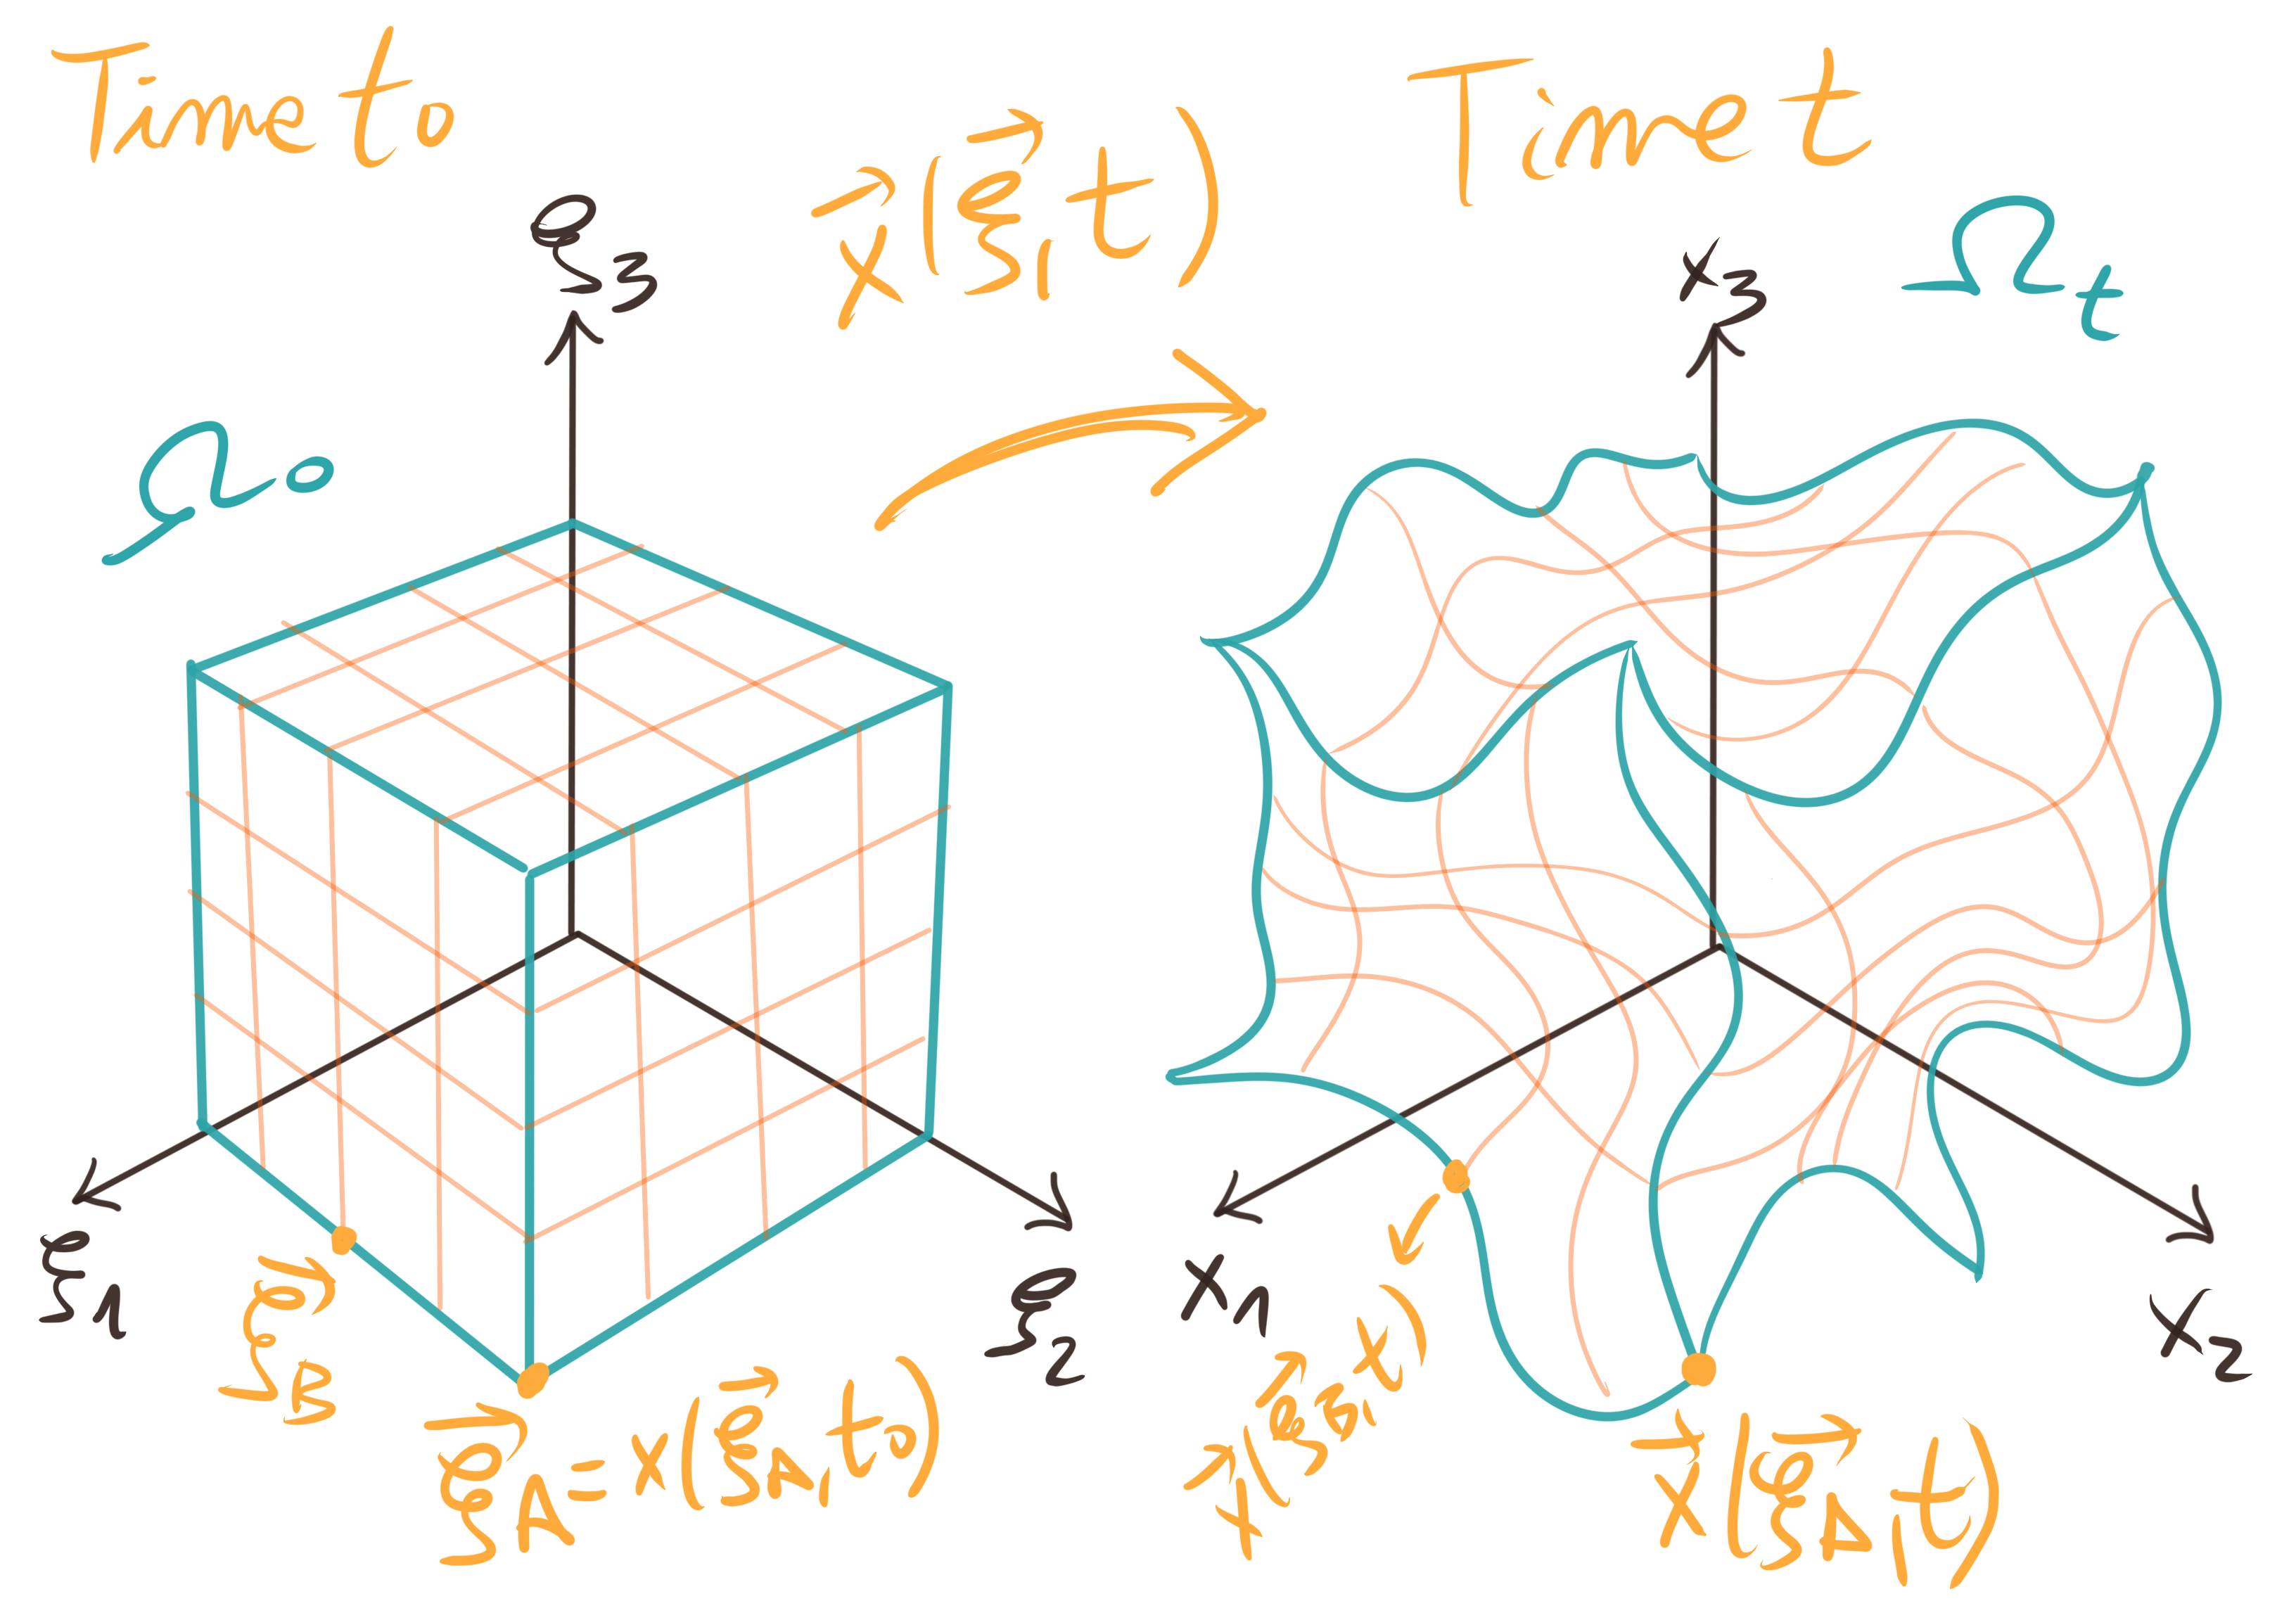
\includegraphics[width=0.57\linewidth]{1deforma.png}
  \caption{Depiction of the $N=3$ case of a homeomorphism representing the trajectory ensemble of a fluid following the notation presented in the text. \vspace{-0.2cm}}
  \label{fig:deform}
\end{figure}

We say that these alternative Universes are {\bf Tangent Universes}, because they can be arbitrarily close to each other in configuration space (that is, the set of positions in physical space for their particles can be arbitrarily similar), but their trajectories never cross each other, meaning they never have the same configuration at the same time.

\newpage
Note now that if we were just given the continuous velocity field for the trajectories of the Universes $\vec{v}\qty(\vec{x}(\vec{\xi},t),t):=\dv{\vec{x}(\vec{\xi},t)}{t}$, we could simply get the ensemble of trajectories by integration.

\begin{equation}
\vec{x}\qty(\vec{\xi},t)=\int_{t_0}^t \vec{v}\qty(\vec{x}(\vec{\xi},t),t)\ dt
\end{equation}
using the initial condition $\vec{x}\qty(\vec{\xi},t_0)=\vec{\xi}$ we have set by definition.

Thus, the velocity field seems to uniquely characterize the trajectory ensemble. This is why it will be one of the properties of the fluid we will look for when trying to define the state of the Tangent Universe Fluid.

There is yet another thing we need to assume to arrive to Quantum Mechanics. The relative amount of Universes in each configuration need not be homogeneous, meaning, we can define the ratio of Universes in a certain configuration, with respect to the total, as a (positive) density function $\rho(\vec{x},t)$, the {\bf density of tangent Universes}. Since we define it to be normalized with respect to the total number of Universes, we assume it integrates to unity in configuration space.

\begin{equation}\label{norm}
\iint_{\Omega_t} \rho(\vec{x},t)\ dx_1\cdots dx_N=1\quad \forall t
\end{equation}

Then, integrating this density in a certain volume $V\subseteq\R^N$ would give us the relative number of Universes with configurations in $V$, which by definition will be a positive real number in the range $[0,1]$.

These two fields in configuration space: the velocity of the trajectory ensemble $\vec{v}(\vec{x},t)$ (defining the ensemble $\vec{x}(\vec{\xi},t)$) and the relative tangent Universe density $\rho(\vec{x},t)$, will completely define the state of the Fluid of Universes at all times.

%\mybox{One could argue that we could also set additional or alternative epistemological or ontological bases, such as the velocity of the degrees of freedom of the Universe, their energy, or any other derived mathematical property. However, it turns out that if we are to measure the velocity of something, we always end up measuring the position of a cursor, even if the cursor was designed to be coupled or causally correlated with the velocity of the measured thing, or alternatively, we end up measuring the position of the thing in different close times and then dividing by the elapsed time increment. In fact, since position is also the ontological basis of classical mechanics, classically interesting properties in last resort are always defined using the position, meaning that in principle it seems that we can always compute properties of interest as derived from the position of the things.

%Note however that fixing the position as epistemological basis of the model does not restrict the ontological basis to be so: the true underlying basic essence of reality could be any other property of the system (as suggest the so called "modal theories"). However, since following the philosophical prologue, in practice there is almost no distinction between what we can consider to be real and the common human phenomenon. Thus, position of things in the phenomenon being so simple to agree on, it seems a reasonable ontology for a model.

%All in all, we choose as the measurable (epistemologically accesible) and underlying (ontological fabric) property, defining the state of our Universe, the space of possible configurations of the degrees of freedom of the Universe in each time. This is what we call the {\bf configuration space} of the Universe in each time.}

\subsection*{A.1.3. The Lagrangian and Eulerian Frames}
\addcontentsline{toc}{subsubsection}{1.3. The Lagrangian and Eulerian Frames}

We can now realize that we will be able to describe a state variable of the fluid, both by reference to a specific configuration-space position $\vec{x}$ at a certain time $t$ or by reference to a specific fluid element (or possible Universe) $\vec{\xi}$ at a certain time. These will be respectively the Eulerian and the Lagrangian frames. 

Given a property $f$ of the fluid (like the density, the velocity or any other derived one), it will be described in the Lagrangian frame if its values are given as seen from the $\vec{\xi}$-th Universe, that is, along the trajectory of that fluid element $f(\vec{x}(\vec{\xi},t),t)$. Alternatively, we could see the value of the properties at each time from a particular fixed Universe configuration $\vec{x}$, as $f(\vec{x},t)$, which would be the Eulerian frame.
 




 
\subsection*{A.1.4. The Measurement Axiom}

\addcontentsline{toc}{subsubsection}{1.4. The Measurement Axiom}
% Why QMs seem to be a non-deterministic theory, where in reality it is! (Since it can be formulated with only unitary deterministic time evolution!)

If we knew $\vec{\xi}\in\R^N$ was the position of every particle of our Universe at an arbitrary single time, say at time $t_0$, we could then deterministically predict the time evolution of our Universe using the trajectory ensemble $\vec{x}(\vec{\xi},t)$. However, knowning the position of every particle in the Universe at the same time is far from being possible. Therefore, we cannot exactly know which of the tangent Universes is ours. From our point of view, the configuration of our Universe is thus an unknown, a random variable. 

Since a priori, we have no information about which of the Universes is ours, we can refer to the tangent Universes as {\bf possible Universes}. A priori then, the best guess we can make is giving the same probability to each of the possible Universes to be ours. As the relative amount of Universes is given by the density $\rho(\vec{x},t)$, which we conveniently decided to normalize to unity, this would mean that we could identify the probability density of the configuration of our Universe with the density of tangent Universes (assigning a same probability to each possible Universe, we will have a weight due to their relative amount). That is, for a domain $V\subseteq \R^N$:
\begin{equation}
P\qty(\text{our Universe has its configuration in }V\text{ at time }t)=P(\vec{x}\in V\ |\ t) := \iint_{V}\rho(\vec{x},t)\ dx_1\cdots dx_N
\end{equation}

If instead we are only interested on the probability that a subset of the particles of our Universe $\vec{y}=(x_1,...,x_m)$ such that $m<N$, have their configuration in $V_y\subseteq \R^m$, we would simply use the marginal probability density derived from the global prior density:
$$
P(\vec{y}\in V_y\ |\ t) := \iint_{V_y}\qty(\iint_{\Omega_t}\rho(\vec{x},t)\ dx_{m+1}\cdots dx_N)dx_1\cdots dx_m
$$
\mybox{
Note that for the introduction of the narrative, we have been saying that ontologically our Universe has a discrete trajectory $\vec{x}(\vec{\xi},t)$, however, since in practice it is not possible to know the position of a particle with infinite precision (since we are dealing with continuous variables and not a variable with a countable support), the tangent Universes we should consider ontologically are those ones weighted by the density $\rho(\vec{\xi},t)$ and not the actual discrete ones. That is to say, the density of Universes will not need to be preserved along the trajectories. Instead they will need to be preserved in subsets of $R^N$ that move along with the trajectories! This is related to the typical discussion on the meaninglessness of observing a discrete value for a continuous probability density variable. We will see the relevance of this when we talk about the local conservation of the amount of Universes in the next section.\\

It is interesting however that this observation opens the question of whether quantum theory is just the continous limit of a more fundamental theory where there is actually a countable number of possible Universes! If their number is very big, most predictions would coincide at a big degree with the theory were there is an uncountable number of Universes. However, they could clearly have different predictions for some very fine experiments. Different predictions that could be perceived in the phenomenon and thus help falsify the underlying theory. It is here where we can see the relevance of a narrative given to a physical theory. It can open ways to search for alternative theories and test non-trivial limits of the current theory. Actually, such an alternative Discrete Tangent Universe Quantum Theory was discussed very recently in Ref. \cite{TangentWiseman} by Wiseman et al.
}

\newpage
\fancyhead[R]{\em The Dynamics of the Universe}
\section*{A.2. The Dynamics of the Universe}
\addcontentsline{toc}{subsection}{2. The Dynamics of the Universe}
% Las ecuaciones dinámicas de la densidad y de la acción. La ecuación de Schrödinger

After understanding the way in which we can define the {\bf state} of the Universal fluid, let us now derive the equations of motion for its defining fields: the density and the velocity fields. For this, we will first derive the equations of motion of the particles in the physical space of each Universe from symmetry considerations about the nature of physical space and time. Then we will introduce the possibility of interaction between different Universes, together with an axiom similar to the Second Law of Thermodynamics, an axiom for the conservation of Universes and one for the total energy. All these together, will lead us directly to the well known Schrödinger Equation, evolving both the configuration-space velocity field and the Universe density at once.

\subsection*{A.2.1. The Stationary Action Axiom within each Universe}

\addcontentsline{toc}{subsubsection}{2.1. The Stationary Action Axiom within each Universe}

Let us first focus on a single Universe of the ensemble of Tangent Universes and the particles observed within the physical space of this single Universe.

Let us denote the degrees of freedom of the $k$-th particle as $\vec{q}_k=(x_{3k-2},\ x_{3k-1},\ x_{3k} )$ with $k\in\{1,...,n\}$, such that we denote the degrees of the ensemble of particles as $\vec{x}=(x_1,...,x_N)\equiv (\vec{q}_{1},...,\vec{q}_n)$.

The {\bf Stationary Action Axiom} within each Universe states that given the boundary values for the trajectory of all the of particles $\vec{x}(t)$ (for a single Universe) are given as $\vec{x}(t_0)=\vec{x}_0$ and $\vec{x}(t_f)=\vec{x}_f$ for some fixed $t_0<t_f\in\R$, $\vec{x}_0, \vec{x}_f\in\R^N$, there exists some function $L(t, \vec{x}, \dv{\vec{x}}{t})$, called the {\bf Lagrangian} of the Universe, such that, the trajectory taken by the ensemble $\vec{x}(t)$, which we call the {\bf physical trajectory}, is that yielding a critical point of the so called {\bf action functional}, which is the integral of the Lagrangian along the positions and velocities taken by the trajectory:
\begin{equation}\label{action}
\s\qty[\vec{x}(t);\ t_0,t_f,x_0, x_f] = \int_{t_0}^{t_f} L\qty(t, \vec{x}(t),\dv{\vec{x}(t)}{t}(t))\ dt
\end{equation}
By a critical point, we mean a trajectory $\vec{x}(t)$ which if perturbed to the valid trajectories closest to it (the ones satisfying the boundaries), yields an action that is a critical point (typically a minimum). That is, we seek for trajectories for which the variation of the action is zero in the locality of the trajectory, that is, we look for trajectories yielding a stationary action.

As we prove in the next gray box, a necessary condition for such a trajectory is to obey the $N$, so called, Euler-Lagrange equations:
\begin{equation}\label{EL}
\pdv{L}{x_j}-\dv{}{t}\pdv{L}{\qty(\dv{x_j}{t})}=0\quad \quad \forall j\in\{1,...,N\}
\end{equation}
These partial differential equations are the so called {\bf equations of motion} of the system, since they define the motion of the trajectory $\vec{x}(t)$.
\mybox{
{\bf Derivation of the Euler-Lagrange Equations}
}

\subsection*{A.2.1.1. The Lagrangian of a Universe from symmetries of physical space and time}

It turns out that the symmetries of the Lagrangian $L$ are transferred to symmetries of the resulting differential equations. This means that if we construct a Lagrangian obeying the postulates about symmetries of the Universe that we prefer, then the resulting laws of motion will obey them as well.

\subsection*{A Single Universe and a Single Particle}
Consider an isolated Universe (from the rest of Universes in the fluid) where there is only one particle, $\vec{x}=\vec{q}$. If there is only one particle (and one Universe), there should not be any influences on its motion, other than the ones caused by the structure of the physical space and time in which it lies.

First of all we will assume the Universal {\bf time} axis is {\bf homogeneous} with respect to the laws of physics: no matter where in time we are, the same equations of motion should work, the laws of physics should be the same. This means that the Lagrangian should be the same for any time shift $\tau$, which in turn can be true if it does not depend explicitly on time:
\begin{equation}\label{tshift}
L\qty(t+\tau,\ \vec{q},\ \dv{\vec{q}}{t})=L\qty(t,\ \vec{q},\ \dv{\vec{q}}{t})\quad \forall t,\tau\in \R \Longrightarrow L\qty(t,\ \vec{q},\ \dv{\vec{q}}{t})=L\qty(\vec{q},\ \dv{\vec{q}}{t})
\end{equation}
\mybox{
Technically, the resulting equations of motion are the same for a Lagrangian and the same Lagrangian with an additive divergence term (with respect to the independent variables), in this case a total time derivative. That is, the Lagrangian $L(t, \vec{q}, \dv{\vec{q}})$ and $L(t, \vec{q}, \dv{\vec{q}})+\dv{}{t}f(t,\vec{q})$ for any "well behaved" function $f$ of time and position, would yield the same equations of motion. We prove this in Appendix $\alpha$ for a general case.\\

This means that for this first symmetry, we would have had enough if:
\begin{equation}
L\qty(t+\tau,\ \vec{q}(t),\  \dv{\vec{q}(t)}{t})=L\qty(t,\  \vec{q},\  \dv{\vec{q}(t)}{t})+\dv{}{t}f(t,\ \vec{q}(t))\quad \forall \tau,t
\end{equation}
for some "well behaved" function $f$ of time and position.\\

However, the simplest Lagrangian could be obtained by further assuming if possible that the Lagrangian itself is invariant under such a symmetry (that is, if $f\equiv0$, as assumed in \eqref{tshift}), which we will assume by Occam's Razor\footnote{If there is a simpler yet equivalent explanation for a same phenomeonon, the simplest one should be preferred. Thus, if a simpler Lagrangian gives us the same equations of motion, we will prefer it over the rest.} for all symmetries but the last one.\\

The same happens for a global multiplicative constant in the Lagrangian. The resulting equations of motion will be the same irrespective of the multiplied global constant.


}
Now, similarly, {\bf physical space} should be {\bf homogeneous}, meaning that wherever we center the coordinate system (apply a shift to the positions), the laws of physics should look the same. This means that we are imposing the Lagrangian to avoid an explicit dependence on the position of the particle:
\begin{equation}
L\qty( \vec{q}+\vec{c}, \dv{\vec{q}}{t})=L\qty( \vec{q}, \dv{\vec{q}}{t})\quad \forall \vec{c},\vec{q}\in \R^3 \Longrightarrow L\qty( \vec{q}, \dv{\vec{q}}{t})=L\qty( \dv{\vec{q}}{t})
\end{equation}
% En + de una particle ojo ke space homogenenous nahi dozu esan +(c,c,c,c) eitzie a (q1,q2,q3,q4)!!!!!!
% The same for rotations! Es la misma rotacion en R3 a cada partícula!

We will also assume the natural axiom that the {\bf physical space} is {\bf isotropic}, meaning that if we rotate the coordinate system, the equations of motion should look the same. Assuming the Lagrangian as well should be invariant, this will avoid the Lagrangian to depend on the direction of the velocities $\dv{\vec{q}}{t}$, leaving it only to depend potentially on their magnitude\footnote{Since $||\dv{\vec{q}}{t}||$ has its image in $[0,\infty)\subset\R$, and $f(s)=s^2$ is a homeomorphism from $[0,\infty)\subset\R$ to itself, we can equivalently consider the dependence on $||\dv{\vec{q}}{t}||$ or on $||\dv{\vec{q}}{t}||^2$ with a little notational abuse for the Lagrangian $L$.} $||\dv{\vec{q}}{t}||^2=\dv{x_1}{t}^2+\dv{x_1}{t}^2+\dv{x_1}{t}^2$. Denoting a rotation of angle $\phi$ about an axis $\vec{u}\in\R^3$ for a vector in $\R^3$ as $Rot(\cdot;\phi, \vec{u})$, we are imposing:
\begin{equation}
L\qty( Rot\qty( \dv{\vec{q}}{t}; phi, \vec{u} ))=L\qty( \dv{\vec{q}}{t})\quad \forall \phi\in\R\ \forall \vec{u}\in \R^3 \Longrightarrow L\qty(\dv{\vec{q}}{t})=L\qty( \Big|\Big|\dv{\vec{q}}{t}\Big|\Big|^2)
\end{equation}
Finally, we will assume {\bf Galilean relativity}. That the equations of motion should be invariant under a constant velocity transformation for the coordinate system. That is, any observer moving at a constant velocity with respect to one another, should observe the same physical laws. This will lead us to conclude that $L\qty( ||\dv{\vec{q}}{t}||^2)=C ||\dv{\vec{q}}{t}||^2$ for some real constant $C$.

To see why, consider an infinitesimal Galilean transformation of the coordinate system by a constant velocity $\vec{\varepsilon}$, with $\vec{\varepsilon}$ in an $\R^3$ ball centered at $\vec{0}$ with an arbitrarily small radious $\delta>0$. Defining $\vec{v}:=\dv{\vec{q}}{t}+\vec{\varepsilon}$, let us expand $L\qty( ||\dv{\vec{q}}{t}+\vec{\varepsilon}||^2)=L(||\vec{v}||^2)$ in power series, centered at $\vec{\varepsilon}=\vec{0}$:
\begin{equation}
L(||\vec{v}||^2)=L\qty(\Big|\Big|\dv{\vec{q}}{t}\Big|\Big|^2)+\pdv{L(||\vec{v}||^2)}{||\vec{v}||^2}\Big\rvert_{\vec{v}=\dv{\vec{q}}{t}}\qty(||\vec{v}||^2-\Big|\Big|\dv{\vec{q}}{t}\Big|\Big|^2)+o\qty(\qty(||\vec{v}||^2-\Big|\Big|\dv{\vec{q}}{t}\Big|\Big|^2)^2  )
\end{equation}
Denoting by $\cdot$ the scalar dot product between two vectors and using that:
\begin{equation}
||\vec{v}||^2-\Big|\Big|\dv{\vec{q}}{t}\Big|\Big|^2=\Big|\Big|\dv{\vec{q}}{t}+\vec{\varepsilon}\ \Big|\Big|^2-\Big|\Big|\dv{\vec{q}}{t}\Big|\Big|^2=\Big|\Big|\dv{\vec{q}}{t}\Big|\Big|^2+||\vec{\varepsilon}||^2+2\vec{q}\cdot \vec{\varepsilon}-\Big|\Big|\dv{\vec{q}}{t}\Big|\Big|^2=2\dv{\vec{q}}{t}\cdot \vec{\varepsilon}
\end{equation}
we get that:
\begin{equation}
L(||\vec{v}||^2)=L\qty(\Big|\Big|\dv{\vec{q}}{t}\Big|\Big|^2)+\pdv{L\qty(||\dv{\vec{q}}{t}||^2)}{||\dv{\vec{q}}{t}||^2}\qty(\dv{\vec{q}}{t}\cdot \vec{\varepsilon})+o\qty(||\vec{\varepsilon}\ ||^2  )
\end{equation}
Since we could choose an arbitrarily small $||\vec{\varepsilon}\ ||^2$, we could take the expression to first order, such that:
\begin{equation}
L\qty(\Big|\Big|\dv{\vec{q}}{t}+\vec{\varepsilon}\ \Big|\Big|^2)=L\qty(\Big|\Big|\dv{\vec{q}}{t}\Big|\Big|^2)+\pdv{L\qty(||\dv{\vec{q}}{t}||^2)}{||\dv{\vec{q}}{t}||^2}\qty(\dv{\vec{q}}{t}\cdot \vec{\varepsilon})
\end{equation}
As it was explained in the last gray-box, this Lagrangian for the Galilean transformation of the coordinate system will lead to the same equations of motion as $L(||\dv{\vec{q}}{t}||^2)$ if the additional term is a total time derivative. That is, if:
\begin{equation}
\pdv{L\qty(||\dv{\vec{q}}{t}||^2)}{||\dv{\vec{q}}{t}||^2}\qty(\dv{\vec{q}}{t}\cdot \vec{\varepsilon})=\dv{f(\vec{q}(t),t)}{t}
\end{equation}
for some arbitrary "well behaved" function $f$ of time and position. If we denote the gradient vector with respect to the variables $\vec{q}$ symbolically as:
\begin{equation}
\vec{\nabla}_{\vec{q}}\equiv(\pdv{}{q_1},\pdv{}{q_2}, \pdv{}{q_3})
\end{equation}
along the trajectory:
\begin{equation}
\pdv{L\qty(||\dv{\vec{q}}{t}||^2)}{||\dv{\vec{q}}{t}||^2}\Big\rvert_{\dv{\vec{q}(t)}{t}}\qty( \vec{\varepsilon}\cdot \dv{\vec{q}(t)}{t})=\pdv{f(\vec{q},t)}{t}\Big\rvert_{\vec{q}(t)}+\vec{\nabla}_{\vec{q}}f(\vec{q},t)\Big\rvert_{\vec{q}(t)}\cdot \dv{\vec{q}(t)}{t}
\end{equation}
The only explicit variable in the left hand side is $\dv{\vec{q}}{t}$, no explicit dependence on $t$ nor $\vec{q}$ beyond it. Therefore, the right hand side will need to behave so, meaning $\pdv{f(\vec{q},t)}{t}$ must be a constant $a$, since a partial derivative in time, of a function of $t$ and $\vec{q}$, can never yield a term as a function of $\dv{\vec{q}(t)}{t}$. For the same reason, $\vec{\nabla}_qf(\vec{q},t)$ will also need to be a constant $\vec{b}$. This means that the left hand side should at most be linear in $\dv{\vec{q}}{t}$, as is the right hand side. Since the $\dv{\vec{q}}{t}$ term is already present in the left hand side, $\pdv{L\qty(||\dv{\vec{q}}{t}||^2)}{||\dv{\vec{q}}{t}||^2}$ will need to be constant. This means that:
\begin{equation}
\pdv{L\qty(||\dv{\vec{q}}{t}||^2)}{||\dv{\vec{q}}{t}||^2}=C \Longrightarrow L\qty(\Big|\Big|\dv{\vec{q}}{t}\Big|\Big|^2) = C\Big|\Big|\dv{\vec{q}}{t}\Big|\Big|^2+c
\end{equation}
for some constants $C,c\in\R$. Since the constant $c$ can be regraded as a total time derivative as well, the resulting equations of motion will be the same setting $c=0$. This would leave the Lagrangian for a free particle as:
\begin{equation}
L\qty(t, \vec{q}, \dv{\vec{q}}{t})=C\Big|\Big|\dv{\vec{q}}{t}\Big|\Big|^2
\end{equation}
We call this term the {\bf kinetic energy} of the particle.

\subsection*{A Single Universe and Many Non-Interacting Particles}

Now, if we had more free particles in this Universe without interaction between them (lets say $n$), we could repeat the space-time symmetry arguments for each of their degrees of freedom and would get that the Lagrangian of the Universe would be a sum of their kinetic energies. The subtle point would be that the constant $C$ would not need to be the same for each particle (we do not have any symmetry telling us so). Thus, the Universe would have a Lagrangian:
\begin{equation}
L\qty(t, \vec{x}, \dv{\vec{x}}{t})=\sum_{k=1}^n C_k\Big|\Big|\dv{\vec{q}_k}{t}\Big|\Big|^2
\end{equation}
Since a Lagrangian will provide the same equations of motion for any non-zero multiplicative global factor, we could establish one of the $C_k=1$ and the rest measure them relative to that one. That is, we could use the constant of one of the particles as a standard $C$ and scale the rest accordingly. This would result in a very particular choice of units, that we will not follow. Instead, for historical reasons, we will write these constants as $C_k=m_k/2$, and call $m_k$ the {\bf mass} of the $k$-th particle. It will represent the restriction of the particle posed on its displacement.

\subsection*{A Single Universe and Many Interacting Particles}

Now, if there was any kind of spatial influence that the position of one particle could exert on the position of the rest, we could model this influence of the $k$-th particle on the $j$-th one as a constraint between their positions, which can in general be modeled by an arbitrary function $V_{kj}(\vec{q}_k, \vec{q}_j)$ added to the free particle Lagrangian. Note that we do not allow an explicit time dependence on this influence term, since time should be homogeneous (the law of their interaction should be constant in time). For reasons that will become clear in a few paragraphs, we will choose to write these arbitrary constraint functions with a negative sign. Such interaction terms for every pair of particles would leave a Universal Lagrangian:
\begin{equation}
L\qty(t, \vec{x}, \dv{\vec{x}}{t})=\sum_{k=1}^n\frac{1}{2}m_k\Big|\Big|\dv{\vec{q}_k}{t}\Big|\Big|^2-\sum_{k<j}V_{kj}(\vec{q}_k, \vec{q}_j)
\end{equation}
We could further simplify it by recurring back to the axioms. Rearranging the position variables of any particle pair $\vec{q}_k$, $\vec{q}_j$ as:
\begin{equation}
\vec{w}_{kj}:=\frac{m_k\vec{q}_k+m_j\vec{q}_j}{m_k+m_j} \quad \vec{r}_{kj}:=\vec{q}_k-\vec{q}_j
\end{equation}
where $\vec{w}_{kj}$ is the center of mass between the particles and $\vec{r}_{kj}$ is their relative position, we could have abusing notation, the influence functions written as $V_{kj}(\vec{w}_{kj}, \vec{r}_{kj})$. Now, translational invariance due to homogeneity of space requires that if the coordinate system is displaced by $\vec{c}\in\R^3$, the Lagrangian is left invariant. Such a translation of the coordinate system would leave the relative position of the particles $\vec{r}_{kj}$ the same, but would displace the gravicenter to $\vec{w}_{kj}+\vec{c}$. This means we would be requiring for the homogeneity of space that $V_{kj}(\vec{w}_{kj}+\vec{c},\vec{r}_{kj})=V_{kj}(\vec{w}_{kj},\vec{r}_{kj})$ $\forall \vec{c}\in\R^3$, which implies $V_{kj}(\vec{w}_{kj},\vec{r}_{kj})$ cannot be a function of $\vec{w_{kj}}$. Leaving $V_{kj}(\vec{w}_{kj},\vec{r}_{kj})=V_{kj}(\vec{r}_{kj})$.

Finally, due to the rotational invariance of the Lagrangian required by the isotropy of space, $V_{kj}(Rot(\vec{r}_{kj};\phi, \vec{u}))=V_{kj}(\vec{r}_{kj})$ for any rotation angle $\phi$ and axis $\vec{u}$. This could only be true if the mutual restriction $V_{kj}$ was exclusively a function of the magnitude $||\vec{r}_{kj}||$ and not its direction. Thus the only allowed potential interaction term should be as a function of the relative distance of the particles $V(||\vec{q}_k-\vec{q}_j||)$. Leaving a total Universe Lagrangian as:\vspace{-0.15cm}
\begin{equation}
L\qty(t, \vec{x}, \dv{\vec{x}}{t})=\sum_{k}\frac{1}{2} m_k\Big|\Big|\dv{\vec{q}_k}{t}\Big|\Big|^2-\sum_{k<j} V_{kj}(\ ||\vec{q}_k-\vec{q}_j||\ )\vspace{-0.15cm}
\end{equation}
Substituting this Lagrangian in the Euler-Lagrange equations \eqref{EL} would leave that the physical trajectory followed by the Universe would need to be given by the system of partial differential equations:
\begin{equation}
m_k \dv[2]{\vec{q}_k(t)}{t} = -\sum_{j\neq k}\vec{\nabla}_{\vec{q}_k} V_{kj}\qty(\ ||\vec{q}_k(t)-\vec{q}_j(t)||\ )\quad\quad \forall k\in\{1,...,n\}\vspace{-0.15cm}
\end{equation}
which is known as {\bf Newton's Second Law} for historical reasons. As such, we identify the interaction terms $V_{kj}(||\vec{q}_k(t)-\vec{q}_j(t)||)$ as the so called {\bf potential energy} terms. The minus sign we introduced was such that we can view the dynamics of this system as the acceleration vector of each particle $\dv[2]{\vec{q}_k(t)}{t} $ pointing towards the minimum of the total potential energy (instead of the maximum). In fact, in classical mechanics, the gradient $\vec{\nabla}_{\vec{q}_k} V_{kj}\qty(\ ||\vec{q}_k(t)-\vec{q}_j(t)||\ )=:\vec{F}_{kj}(\vec{q}_k(t);\ \vec{q}_j(t))$ is called the {\bf force} exerted by the particle $j$ on the $k$-th.

% More conveniently % en plan configuration space al dala exprese tal ke así, pam!


% Oin sería introducir la opción de que diferentes Universos se afecten entre ellos en función de la densidad de Universos. Introduces el potencial Q() incluso podrías justificar que sea en función de rho/xi, x/xi, y podrías demostrar que sigue cumpliendo que el espacio sea tal y cual...o no
% Oin sería introducir el momento y el desarrollo para tener la Hmailton principal function, y decir lo conveniente que es para una posición incial y tiempo inicial dado.
% cuando lo tengas mete el postulado de Fisher Information y de que el potencial cuántico sea cte. y optimiza el meta lagrangiano del universo para obtener las eqt of motion que querías.
% haz muchas más sub-secciones xD
% Y lo de la masa en el Q...bueno, ya veremos. Podrzias intentar justificarlo mirando back a cuando tenías un Universo de una sola partícula. Igualmente igual alzu intente justifiketan Q-ren dependentzixe de isotropy etc. 
% Ta arregle notaziñoko barrak tu eske vaya bazofia jajaj

% direction of time is not defined!!!!
% Introduce un potential energy term for influences that could come from outside the Universe
\vspace{-0.3cm}
\subsection*{An influence in the motion of the Universe by external factors (like other Universes)}
Let us now loosen the assumption that the dynamics of the Universe (the motion of its particles) is only due to the properties of its space-time and the positions of its particles, and introduce the option to have some external factor to this Universe affect the dynamics inside it. This external factor should affect the trajectory of the Universe as a function of where its particles are, and it could actually vary in time for more generality. We could include such an influence by an arbitrary function $-Q(\vec{x},t)$ of the positions and time in the Lagrangian (the minus sign would be just a convenience for having Newton's second law allow us interpret it as a potential energy). This would leave the Universe Lagrangian as:
\begin{equation}\label{genLag}
L\qty(t, \vec{x}, \dv{\vec{x}}{t})=\sum_{k=1}^n\frac{1}{2} m_k\Big|\Big|\dv{\vec{q}_k}{t}\Big|\Big|^2-\qty[\sum_{k<j} V_{kj}(\ ||\vec{q}_k-\vec{q}_j||\ )+Q(\vec{q}_1,...,\vec{q}_N,t)]
\end{equation}
Let us call $Q(\vec{x},t)$ the {\bf external potential energy}. The equations of motion given by \eqref{EL} would then be:\vspace{-0.15cm}
\begin{equation}\label{NewtOneUn}
m_k \dv[2]{\vec{q}_k(t)}{t} = -\vec{\nabla}_{\vec{q}_k}\qty[\sum_{j\neq k} V_{kj}\qty(\ ||\vec{q}_k-\vec{q}_j||\ )+ Q(\vec{q}_1,...,\vec{q}_N,t)]\Big\rvert_{\vec{q}=\vec{q}(t)}\quad\quad \forall k\in\{1,...,n\}
\end{equation}
For simplicity we could actually define a {\bf total potential energy} function $U$ as:
\begin{equation}
U(\vec{x},t):=\sum_{k<j} V_{kj}(\ ||\vec{q}_k-\vec{q}_j||\ )+Q(\vec{q}_1,...,\vec{q}_N,t)\vspace{-0.15cm}
\end{equation}
Having the packs of degrees of freedom for a same particle $\vec{q}_k$ jiggling around is a bit cumbersome. For notational ease we will just write it all for each individual degree of freedom $x_k$. This would leave us the Lagrangian and equations of motion for the Universe as:
\begin{equation}\label{genLag2}
L\qty(t, \vec{x}, \dv{\vec{x}}{t})=\sum_{k=1}^N\frac{1}{2} m_k\qty(\dv{x_k}{t})^2-U(\vec{x},t)
\end{equation}
\begin{equation}
m_k \dv[2]{x_k(t)}{t} = -\pdv{}{x_k}U(\vec{x},t)\Big\rvert_{\vec{x}=\vec{x}(t)}\quad\quad \forall k\in\{1,...,N\}
\end{equation}
where we identify the masses of the same particle $m_{3j}=m_{3j-1}=m_{2j-2}$ for $j\in\{1,...,n\}$.
\mybox{
Note now that in reality the external potential could be seen as the potential for a bigger system in which we forget about the things that are not the Universe of interest. That is, imagine for instance, that we have two Universes that interact between them, an alpha Universe of trajectory $\vec{x}^\alpha(t)=(x_1^\alpha(t),...,x_N^\alpha(t))$ and a beta Universe of trajectory $\vec{x}^\beta(t)=(x_1^\beta(t),...,x_M^\beta(t))$, with $N$, $M$ not necessarily the same numbers (allowing them to have a different number of particles $n=N/3$ and $m=M/3$). A potential of interaction between them, that depended on the positions of one and the other one alone, could be introduced in the joint Lagrangian for the two Universes as a function $Q(\vec{x}^\alpha, \vec{x}^\beta)$ of their positions. Since time is homogeneous, we assume no explicit time dependence on their interaction term. The total Lagrangian would be:
\begin{equation}
L\qty(t, \vec{x}^\alpha, \dv{\vec{x}^\alpha}{t}, \vec{x}^\beta, \dv{\vec{x}^\beta}{t})=\sum_{k=1}^n\frac{1}{2} m^\alpha_k\Big|\Big|\dv{\vec{q}^\alpha_k}{t}\Big|\Big|^2+\sum_{k=1}^m\frac{1}{2} m^\beta_k\Big|\Big|\dv{\vec{q}^\beta_k}{t}\Big|\Big|^2-
\end{equation}
$$
-\qty[\sum_{k<j} V^\alpha_{kj}(\ ||\vec{q}^\alpha_k-\vec{q}^\alpha_j||\ )+\sum_{k<j} V^\beta_{kj}(\ ||\vec{q}^\beta_k-\vec{q}^\beta_j||\ )+ Q(\vec{x}^\alpha, \vec{x}^\beta)]
$$

With the equations of motion for each Universe $\vartheta\in\{\alpha, \beta\}$ being left as:
\begin{equation}
m_k \dv[2]{\vec{x}^\vartheta(t)}{t} = -\vec{\nabla}_{\vec{x}^\vartheta}\qty[\sum_{j< k} V^\vartheta{kj}(\ ||\vec{q}^\vartheta_k-\vec{q}^\vartheta_j||\ )+ Q(\vec{x}^\alpha, \vec{x}^\beta)]{\Bigg\rvert}\null_{  \footnotesize    \begin{array}{r@{}}
\vec{x}^\alpha=\vec{x}^\alpha(t)\\\vec{x}^\beta=\vec{x}^\beta(t) \end{array}}\quad\quad \vartheta\in\{\alpha, \beta\}
\end{equation}
Then, if we simply wanted to forget about the existence of the Universe $\beta$ and only contemplate the dynamics of $\alpha$, since the gradient is only on the degrees of freedom of the Universe of interest, we could directly evaluate the trajectory of the uninteresting Universe, such that:
\begin{equation}\label{trick1}
\vec{\nabla}_{\vec{x}^\alpha}Q(\vec{x}^\alpha, \vec{x}^\beta){\Big\rvert}\null_{  \footnotesize    \begin{array}{r@{}}
\vec{x}^\alpha=\vec{x}^\alpha(t)\\\vec{x}^\beta=\vec{x}^\beta(t) \end{array}}=\vec{\nabla}_{\vec{x}^\alpha}Q(\vec{x}^\alpha, \vec{x}^\beta(t)){\Big\rvert}\null_{ \vec{x}^\alpha=\vec{x}^\alpha(t) }
\end{equation}
where we could then write with a notational abuse:
\begin{equation}\label{trick2}
Q(\vec{x}^\alpha, \vec{x}^\beta(t))=Q(\vec{x}^\alpha, t)
\end{equation}
Which is the "external influence" potential we introduced. Leaving an equation of motion for the $\alpha$-th Universe as:
\begin{equation}
m_k \dv[2]{\vec{x}^\alpha(t)}{t} = -\vec{\nabla}_{\vec{x}^\alpha}\qty[\sum_{j< k} V^\vartheta{kj}(\ ||\vec{q}^\alpha_k-\vec{q}^\alpha_j||\ )+ Q(\vec{x}^\alpha,t)]{\Bigg\rvert}\null_{
\vec{x}^\alpha=\vec{x}^\alpha(t)}
\end{equation}
which is exactly the equation of motion (and Lagrangian) we had in equation \eqref{NewtOneUn}.\\

In fact, we could also introduce interaction potentials between an arbitrary number of Universes and we would be able to do the same trick of equations \eqref{trick1} and \eqref{trick2} to get the external potential shape. Not only that, but we could introduce a collective interaction between all the Universes, as a potential depending on the trajectories of all of them, even for a continuity of Universes, in a way that from the perspective of each single Universe, the influence would still look like a simple external potential in time $Q(\vec{x}^\alpha,t)$. It is this why we are not dropping the homogeneity of the global time axis $t$ by introducing the external potential that can depend on time. It is the {\bf laws of physics for the fluid of Universes that have the same shape under time translations} (not each single Universe!). It would happen the same if we only considered one particle in a Universe with more than one particle interacting with the considered one. From the perspective of the single particle there would be an external time dependent potential, making time seem to be inhomogeneous. It must be the time of the outermost system (the most global perspective) for which time is homogeneous.
}

% Introdyce un potential ke influencia desde fuera del Universo el movimiento de las partículas!!!!
Now, in order to have the velocities of the possible trajectories and their energies all gathered in a same function, we will need to introduce some additional notation delving around with the Lagrangian. This will be a convenient way in which we will have enough with a single function to define the dynamic state of all the Tangent Universes. It will be possible by introducing two alternatives to the raw Euler-Lagrange equations that gave us Newton's Second Law. One will be the momentum and the Hamiltonian formalism, and the other will be the Hamilton-Jacobi action function.

\subsubsection*{A.2.1.2. The Momentum and the Hamiltonian (the Total Energy of a Universe)}
First of all, let us define what we will call the {\bf momentum} of the $k$-th degree of freedom of the Universe. It is the partial derivative of the Lagrangian with respect to the velocity of the $k$-th degree of freedom. That is:
\begin{equation}
p_k\qty(t,\vec{x},\dv{\vec{x}}{t}):=\pdv{L(t,x,\dv{x_k}{t})}{\dv{x_k}{t}}
\end{equation}
Evaluating the most general Lagrangian for a Universe that we got, equation \eqref{genLag} or \eqref{genLag2}, we see that the $k$-th momentum is only a function of the $k$-th velocity for this Lagrangian:
\begin{equation}\label{mom}
p_k\qty(\dv{x_k}{t})=m_k\dv{x_k}{t}
\end{equation}
Now, since the Lagrangian is a quadratic function with respect to any of the velocities $\dv{x_k}{t}$ (the potentials do not depend on velocity explicitly), it has a positive second partial derivative with respect to velocity. This means that the first partial derivative of the Lagrangian with respect to these velocities is a monotonically increasing function (strictly increases), implying that there is a one to one (and continuous) correspondence between the derivative of the Lagrangian with respect to a velocity (the momentum $p_k$) and the value of the velocity $\dv{q_k}{t}$. That is, by fixing the rest of variables, for each momentum $p_k$ there is a single velocity variable $\dv{x_k}{t}$ and vice-versa. This means that the relation in equation \eqref{mom} can be used as a change of variables: there exists an expression to get the momentum from the velocity $p_k(\dv{x_k}{t})$ and an inverse  expression $\dv{\vec{x}}{t} (p_k)$, to get the velocity from  the value of the momentum. In our case the relation is very simple indeed:
\begin{equation}
p_k\qty(\dv{x_k}{t})=m_k\dv{x_k}{t}\quad \quad \dv{x_k}{t} (p_k)=\frac{1}{m_k}p_k
\end{equation}
The momentum is just the velocity times the mass.

We could now define the Lagrangian as a function of the momentum by simply evaluating $\dv{x_k}{t}=\dv{\vec{x}}{t} (p_k)$. Instead however, we are looking for a function $H(t, \vec{x}, \vec{p})$ such that the derivative with respect to the $k$-th momentum, evaluated in $p_k(\dv{x_k}{t})$ gives us back the velocity $\dv{x_k}{t}$. This is, we are looking for a sort of reciprocal function of the Lagrangian with respect to this transformation. The function fulfilling this property is the so called {\bf Hamiltonian} of the Universe:
\begin{equation}
H(t, x_1,...,x_N,p_1,...,p_N):=\sum_{k=1}^N p_k \dv{x_k}{t}  (p_k)-L(t, x_1,...,x_N, \dv{x_1}{t} (p_1),... \dv{x_N}{t} (p_N))
\end{equation}
You can check with the chain rule that this and the Lagrangian are the functions relating the momenta and the velocity by their slopes. That is:
\begin{equation}\label{p1}
\pdv{H}{p_k}=\dv{x_k}{t}(p_k)\quad \text{and}\quad \pdv{L}{\dv{x_k}{t}}=p_k\qty(\dv{x_k}{t})
\end{equation}
We call this transformation that gives us the Hamiltonian from the Lagrangian and vice-versa, the {\bf Legendre transformation} with respect to the velocity or the momentum. Note that this transformation is defined such that it is its own inverse: the Hamiltonian is the Legendre transformation of the Lagrangian with respect to the velocities, and the Lagrangian is the Legendre transformation of the Hamiltonian with respect to the momentum. The interest of such a transformation is that the Hamiltonian formalism with the momentum and positions instead of velocities and positions, gives us an alternative set of equations of motion to those ones offered by the Euler-Lagrange equations as follows.

If we take the partial derivative of the Hamiltonian with respect to the $k$-th position, we find:
\begin{equation}
\pdv{H}{x_k}=\pdv{}{x_k}\qty(\sum_{k=1}^N p_k \dv{x_k}{t} (p_k)-L\qty(t, x_1,...,x_N, \dv{x_1}{t} (p_1),... \dv{x_N}{t} (p_N)))=-\pdv{L}{x_k}
\end{equation}
Now, the physical trajectory (the one extremizing the action) needed to obey the Euler-Lagrange equations \eqref{EL}, where we can find what $\pdv{L}{x_k}$ must be equal to for that. Introducing it in the last expression and applying the definition of $k$-th momentum we get:
\begin{equation}\label{p2}
\pdv{H}{x_k}=-\dv{}{t}\pdv{L}{(\dv{x_k}{t})}=-\dv{}{t}p_k
\end{equation}
Gathering equations \eqref{p1} \eqref{p2}, we have that instead of using the Euler-Lagrange equations to evolve the trajectory in time $\vec{x}(t)$, we could use the so called {\bf Hamiltonian equations}, that will provide us an equivalent trajectory in the so called phase space $(\vec{x}(t), \vec{p}(t))$:
\begin{equation}\label{ham}
\pdv{H(t,\vec{x}(t),\vec{p}(t))}{p_k}=\dv{x_k(t)}{t}\quad\quad \pdv{H(t,\vec{x}(t),\vec{p}(t))}{x_k}=-\dv{p_k(t)}{t}\quad \quad k\in\{1,...,N\}
\end{equation}
The practical advantage of these equations in front of the Euler-Lagrange equations (which should yield the same solutions), is that while the Euler-Lagrange equations are $N$ second order differential equations, Hamilton's equations are $2N$ first order differential equations, which might provide a better insight in some problems. In particular, if a coordinate $x_k$ does not appear in the Hamiltonian, its corresponding momentum is conserved in time by the second Hamilton's equation of \eqref{ham}: thus the coordinate can be ignored in the other equations, effectively reducing the number of equations to $2N-2$. In the Lagrangian formalism on the other hand, if some momentum is conserved, the velocities in the Lagrangian might still occur, avoiding it to reduce the number of equations to be solved.

Aside from this practical point, the Hamiltonian has also a very interesting feature: it is the definition of the {\bf total energy} of the system in a given time, configuration and momentum. For the most general Lagrangian we got from equation \eqref{genLag2}, we have that the Hamiltonian is:
\begin{equation}\label{HamDef}
H(t, \vec{x},\vec{p}\ )=\sum_{k=1}^N \frac{p_k}{2m_k}^2+U(\vec{x},t)=\sum_{k=1}^N \frac{p_k}{2m_k}^2+\sum_{j>k} V_{kj}(\ ||\vec{q}_k-\vec{q}_j||\ )+Q(\vec{x},t)
\end{equation}
which using that $p_k=m_k\dv{x_k}{t}$ can be seen to be the sum of the total kinetic and potential energies (inter-particle and external ones). That is why we called those terms as "energies" in the first place!

\subsection*{A.2.1.3. Introducing the Hamilton-Jacobi Action function}
It turns out that even if the action functional for an optimal path \eqref{action} is complicated to be computed analytically, we can still compute the variation of the action in front of variations of the end point of the physical trajectory in space or time (the point $\vec{x}_f$ or $t_f$).

Let us name the physical trajectory for the end-points $\vec{x}(t_0)=\vec{x}_0$ and $\vec{x}(t_f)=\vec{x}_f$ as $\vec{x}_{old}(t)$. Let us now consider what happens if we slightly {\bf vary the end position} of the trajectory $\vec{x}_f$ to $\vec{x}_f+\Delta\vec{x}$, with $\Delta\vec{x}_f=(\Delta x_{1_f}, ..., \Delta x_{N_f})$ a vector of small displacements in configuration space $\R^N$. If we keep fixed the starting point $\vec{x}(t_0)=\vec{x}_0$, the new trajectory for the Universe will be the previous physical one $\vec{x}_{old}(t)$ plus a variation $\delta \vec{x}(t)=(\delta x_1(t),...,\delta x_N(t))$ at each time, such that the new trajectory $\vec{x}(t)=\vec{x}_{old}+\delta \vec{x}(t)$ will have $\delta \vec{x}(t_0)=0$ and $\delta \vec{x}(t_f)=\Delta\vec{x}$. If we now expand the Lagrangian in Taylor series for the trajectory $\vec{x}(t)=\vec{x}_{old}(t)+\delta\vec{x}(t)$ (such that $\dv{\vec{x}}{t}(t)=\dv{\vec{x}_{old}}{t} (t)+\dv{}{t}\delta \vec{x}(t)$), centered at the trajectory $\vec{x}_{old}(t)$, we have that:
\begin{equation}
L\qty(t, \vec{x}(t), \dv{\vec{x}(t)}{t})=L\qty(t, \vec{x}_{old}(t), \dv{\vec{x}_{old}(t)}{t})+\sum_{k=1}^N \pdv{L\qty(t, \vec{x}, \dv{\vec{x}}{t})}{x_k}\Big\rvert_{\vec{x}_{old}(t)}\qty(x_k(t)-x_{k_{old}}(t))+
\end{equation}
$$
+\sum_{k=1}^N \pdv{L\qty(t, \vec{x}, \dv{\vec{x}}{t})}{\dv{x_k}{t}}\Big\rvert_{\vec{x}_{old} (t)}\qty(\dv{}{t}x_k(t)-\dv{}{t}x_{k_{old}}(t))+
o\qty(||\vec{x}(t)-\vec{x}_{old}(t)||^2+||\dv{\vec{x}}{t} (t)-\dv{\vec{x}_{old}}{t} (t) ||^2)=
$$
$$
=L\qty(t, \vec{x}_{old}(t), \dv{\vec{x}_{old}(t)}{t})+\sum_{k=1}^N \qty{\pdv{L\qty(t, \vec{x}, \dv{\vec{x}}{t})}{x_k}\Big\rvert_{\vec{x}_{old}(t)}\delta x_k(t)+\pdv{L\qty(t, \vec{x}, \dv{\vec{x}}{t})}{\dv{x_k}{t}}\Big\rvert_{\vec{x}_{old}(t)}\dv{}{t}\delta x_k(t)}
$$
$$
+o\qty(||\delta\vec{x}(t)||^2+||\dv{\delta \vec{x}(t)}{t}||^2)
$$
Since the displacement of the end-point $\Delta \vec{x}_f$ can be taken arbitrarily small, the variation in the action between the old and the new trajectory (differing in their end points) will then be given to first order by:
\begin{equation}
\Delta \s:=\s[\vec{x}(t)]-\s[\vec{x}_{old}(t)]=\int_{t_0}^{t_f} L\qty(t, \vec{x}(t), \dv{\vec{x}}{t})\ dt - \int_{t_0}^{t_f} L\qty(t, \vec{x}_{old}(t), \dv{\vec{x}}{t})\ dt=
\end{equation}
$$
= \int_{t_0}^{t_f}  \sum_{k=1}^N \qty{\pdv{L\qty(t, \vec{x}, \dv{\vec{x}}{t})}{x_k}\Big\rvert_{\vec{x}_{old}(t)}\delta x_k(t)+\pdv{L\qty(t, \vec{x}, \dv{\vec{x}}{t})}{\dv{x_k}{t}}\Big\rvert_{\vec{x}_{old}(t)}\dv{}{t}\delta x_k(t)}
\ dt
$$
Since $\vec{x}_{old}(t)$ is a physical trajectory, it follows the Euler-Lagrange equations \eqref{EL}, meaning we can evaluate $\pdv{L}{x_k}$ to get:
\begin{equation}
\Delta \s=\int_{t_0}^{t_f}  \sum_{k=1}^N \qty{\dv{}{t}\qty(\pdv{L\qty(t, \vec{x}, \dv{\vec{x}}{t})}{\dv{x_k}{t}}\Big\rvert_{\vec{x}_{old}(t)})\delta x_k(t)+\pdv{L\qty(t, \vec{x}, \dv{\vec{x}}{t})}{\dv{x_k}{t}}\Big\rvert_{\vec{x}_{old}(t)}\dv{}{t}\delta x_k(t)}
\ dt=
\end{equation}
$$
= \sum_{k=1}^N \int_{t_0}^{t_f} \dv{}{t}\qty(\pdv{L\qty(t, \vec{x}, \dv{\vec{x}}{t})}{\dv{x_k}{t}}\Big\rvert_{\vec{x}_{old}(t)}\delta x_k(t))
\ dt=
$$
$$
=\sum_{k=1}^N\qty[\pdv{L\qty(t, \vec{x}, \dv{\vec{x}}{t})}{\dv{x_k}{t}}\Big\rvert_{\vec{x}_{old}(t)}\delta x_k(t)]^{t_f}_{t_0}=\sum_{k=1}^N\pdv{L\qty(t, \vec{x}, \dv{\vec{x}}{t})}{\dv{x_k}{t}}\Big\rvert_{\vec{x}(t_f)}\Delta x_{k_f}
$$
where we used the derivative of a product rule and the fact that $\delta \vec{x}(t_f)=\Delta \vec{x}_f$ and $\delta \vec{x}(t_0)=0$.

Now, choosing the displacement to be $\Delta x_{j_f}=0$ $\forall j\neq k$:
\begin{equation}
\frac{\Delta \s(\vec{x}_f)}{\Delta x_{k_f}}=\pdv{L\qty(t, \vec{x}, \dv{\vec{x}}{t})}{\dv{x_k}{t}}\Big\rvert_{\vec{x}(t_f)}=:p\qty(\dv{\vec{x}(t_f)}{t})
\end{equation}
As we make the limit $\Delta x_{k_f}\rightarrow 0$, we get that the first order approximation we made will be an exact equality and that:
\begin{equation}\label{momS}
\pdv{S(\vec{x},t)}{x_k}=p_k(t)
\end{equation}
where we defined the {\bf Hamilton-Jacobi action function} as:
\begin{equation}
S(\vec{x},t):=\int_{t_0;\ \vec{x}_0}^{t; \ \vec{x}} L\qty(\tau, \vec{x}(\tau),\dv{\vec{x}(\tau)}{t} )\ d\tau
\end{equation}
with $t_0$ and $\vec{x}_0$ are fixed undetermined constants and $\vec{x},t$ representing the final end-point of the trajectory.

Equation \eqref{momS} means that the variation in the action with respect to space, gives the momentum field (and thus velocity field) for the physical trajectories.

Finally, let us understand what happens if we {\bf vary the end time} of the trajectory by an arbitrarily small amount $\Delta t$ (ensuring that the same point $\vec{x}_f$ is crossed at time $t_f$):
\begin{equation}
\Delta \s[t_f]:=\s[\vec{x}(t); \vec{x}(t_f),t_f]-\s[\vec{x}(t); \vec{x}(t_f+\Delta t), t_f+\Delta t]=\int_{t_0}^{t_f+\Delta t} L\qty(t, \vec{x}(t), \dv{\vec{x}}{t})\ dt - \int_{t_0}^{t_f} L\qty(t, \vec{x}(t), \dv{\vec{x}}{t})\ dt
\end{equation}
$$
\lim_{\Delta t\rightarrow 0}\Delta \s[t_f]= \lim_{\Delta t\rightarrow 0}\int_{t_f}^{\Delta t} L\qty(t, \vec{x}(t), \dv{\vec{x}}{t})\ dt=\lim_{\Delta t\rightarrow 0}  L\qty(t_f, \vec{x}(t_f), \dv{\vec{x}}{t_f})\Delta t
$$
where we used the definition of integral as a limit of Riemann sums. Then, these would leave:
\begin{equation}
\lim_{\Delta t\rightarrow 0}\qty(\frac{\Delta \s[t_f]}{\Delta t} )= L\qty(t_f, \vec{x}(t_f), \dv{\vec{x}}{t_f})
\end{equation}
such that:
\begin{equation}\label{azk}
\dv{S(\vec{x},t)}{t}=L(t,\vec{x},\dv{\vec{x}}{t})
\end{equation}
Now, using that along the trajectory $\vec{x}(t)$ by the chain rule:
\begin{equation}
\dv{S(\vec{x}(t),t)}{t} = \pdv{S(\vec{x}(t),t)}{t}+\sum_{k=1}^N\pdv{S(\vec{x},t)}{x_k}\Big\rvert_{\vec{x}(t)}\dv{x_k(t)}{t}
\end{equation}
and using that if the trajectory $\vec{x}(t)$ is a physical trajectory, following the Euler-Lagrange equations, then equations \eqref{momS} and \eqref{azk} hold, we can evaluate them here to get:
\begin{equation}
L\qty(t, \vec{x}(t), \dv{\vec{x}(t)}{t})=\pdv{S(\vec{x}(t),t)}{t}+\sum_{k=1}^N p_k\qty(\dv{x_k(t)}{t})\dv{x_k(t)}{t}
\end{equation}
By writing the velocity as a function of the momentum $\dv{\vec{x}}{t} (\vec{p})$ and rearranging terms, we can see that suddenly the Hamiltonian emerges back:
\begin{equation}
-\pdv{S(\vec{x}(t),t)}{t}=\sum_{k=1}^N p_k\dv{x_k}{t} (p_k(t))-L\qty(t, \vec{x}(t), \dv{\vec{x}(\vec{p}(t))}{t})=H(t, \vec{x}(t), \vec{p}(t))
\end{equation}
Thus leaving that:
\begin{equation}\label{hamS}
\pdv{S(\vec{x},t)}{t}=-H(t, \vec{x}, \vec{p})
\end{equation}
which means that the variation of the action if we move a time step along the trajectory is (minus) the energy of the Universe at that time.

The two equations \eqref{momS} and \eqref{hamS}, lead us to a third way to get the motion of the Universe:
\begin{equation}\label{HJE}
\pdv{S(\vec{x},t)}{t}=-H\qty(t, \vec{x}, \vec{p}=\vec{\nabla}_{x}S(\vec{x},t))
\end{equation}
which lets us evolve the field $S(\vec{x},t)$ given an initial relative action field $S(\vec{x},t_0)=s_0(\vec{x})$. This is called the {\bf Hamilton-Jacobi equation}. 

Note that when solving this equation, one cannot simply evolve a single trajectory, as allowed us the Euler-Lagrange (Newton's law) and Hamilton's equations. Instead, we here evolve a field in configuration space $S(\vec{x},t)$, the spatial derivative of which will provide us the momentum and thus velocity field to evolve the trajectories. That is, solving the Hamilton-Jacobi equation means getting all the possible trajectories of the system provided a relative initial action field. This is why it is not typically employed as a practical tool for calculations, since normally we are only interested in getting a single trajectory for the system, and not all the possible trajectories. It turns out however, that this will be the perfect tool for evolving all the trajectories of the different Universes at once! Thus the relevance of its introduction for us to arrive to quantum mechanics.

\subsection*{A.2.2. The Stationary Action Axiom at the Universe Fluid level}

\addcontentsline{toc}{subsubsection}{2.2. The Stationary Action Axiom at the Universe Fluid level}

The equations until now assumed that if there were more than one Universes they were not able to interact with each other. We have found that within each of these non-interacting Universes, the trajectory of their particles was predictable by just knowing the position of the particles at any particular time and integrating any of the shapes for the equations of motion we derived (most conveniently the Euler-Lagrange or Hamilton's equations). 

Now, let us explicitly introduce the assumption that in the locality of any possible configuration $\vec{x}\in\Omega_t\subseteq\R^N$, there are $\rho(\vec{x},t)dx_1\cdots dx_N$ actual physical Universes with the {\bf same number of particles and relative interaction potentials}, with their physical spaces having the {\bf same symmetries} as the ones required to derive the equations of motion of the previous sections. If all these conditions were the same for each of the Universes, the equations of motion for all of them would be the same as well, and would only depend on their initial configurations. This would also make them all have the same Lagrangian and action functional, and all of them would have {\bf the same Hamilton-Jacobi action} $S(\vec{x},t)$. The derivative $\pdv{S(\vec{x},t)}{x_k}$ would yield {\bf the same} field of momentums and velocities for their possible physical trajectories, by equation \eqref{momS}. The derivative $-\pdv{S(\vec{x},t)}{t}$ would yield {\bf the same} total energy for a trajectory at $\vec{x}$ and time $t$, of any of the Universes, due to equation \eqref{hamS}.

Now, if we assume that each Universe has a different and defined configuration $\vec{\xi}$ at a time $t_0$, we will have that the single {\bf same} action function $S(\vec{x},t)$ will encode the velocity and total energy fields (and thus the trajectories) of all the different Universes. As was stated in the introduction, we will express these trajectories with a function $\vec{x}(\vec{\xi},t)$, where the label $\vec{\xi}$ tags the trajectory that was at $\vec{\xi}$ at time $t_0$. That is, using that $\vec{x}(\vec{\xi},t_0)=\vec{\xi}$. 

Since all Universes have the same $S(\vec{x},t)$, we will be able to get the different trajectories by integrating the same velocity field for each of the different $\vec{\xi}$. We can get this velocity field by inverting the relation between the momentum and the velocity:
\begin{equation}\label{GL}
\dv{x_k(\vec{\xi},\,t )}{t} =v_k(\vec{x}(\vec{\xi},t),t)=\frac{1}{m_k}p_k\qty(\dv{x_k(\vec{\xi},\,t )}{t})= \frac{1}{m_k} \pdv{S(\vec{x},t)}{x_k}\Big\rvert_{\vec{x}=\vec{x}( \vec{\xi},t)}\quad \forall k\in\{1,...,N\}
\end{equation}
Defining the velocity field for the fluid of Universes as:
\begin{equation}\label{v}
v_k(\vec{x}(\vec{\xi},t),t):= \frac{1}{m_k} \pdv{S(\vec{x},t)}{x_k}\Big\rvert_{\vec{x}=\vec{x}( \vec{\xi},t)}
\end{equation}

In short, we will have enough with a single field $S(\vec{x},t)$ to encode the trajectories of all the Universes.


\mybox{
If we leave a null external potential $Q(\vec{x},t)\equiv 0$, the narrative till this point would be a valid interpretation of classical mechanics. This interpretation would be a bit convoluted because it would be saying that there are infinite {\bf parallel} Universes ({\bf not tangent}, since they do not interact and thus could cross each other like ghosts). The only interest of this narrative would be that since we do not know which exactly are our "initial" conditions, computing all the possible trajectories $\vec{x}(\vec{\xi},t)$ would be helpful. To reflect this uncertainty we could introduce a probability density, that according to this interpretation could be seen as a density of parallel Universes $\rho(\vec{x},t)$. Evolving the density with a continuity equation, we would have a stochastic classical mechanics theory. \\

However, since the density would not be able to affect the trajectories of the Universes, as it appears no-where in the equations of motion, the "only one version of reality" interpretation would work as fine as the parallel Universe interpretation. So there would be no need to say that the probability density is in reality the density of parallel Universes. If we see no effect of the parallel Universes in the motion of ours, why to assume their existence? By Occam's Razor, we would clearly prune this overcomplicated interpretation.\\

It will turn out in quantum mechanics however, that the density will affect contingently each trajectory, such that from any of the Universes the pushing effect of the rest could be physically perceived. It is this why in quantum mechanics, a {\bf tangent} Universe interpretation will be the most natural one, against an interpretation where "possible but non-existent" realities affect the perceived one, which is clearly non-sense.
}

Note how for now nothing seems to avoid the trajectories $\vec	{x}(\vec{\xi},t)$ to get multivalued (to cross each other at the same time). The "univalued-ness" will be ensured by the fact that we will assume {\bf $S$ is differentiable with continuous first derivatives}\footnote{Lipschitz-continous in $\vec{x}$ and continous in $t$.}, such that the momentum and thus the velocity field $\vec{v}(\vec{x},t)$ for the trajectories, defined in equation \eqref{v}, will be {\bf continuous}. Then, by the Picard-Lindelöf theorem for the existence and uniqueness of the initial value problem \eqref{GL}, the trajectories will exist and will be unique for a given initial condition. This means that just a single trajectory will cross each configuration-space and time point at the same time. 


Finally, let us explicitly introduce the possibility for the trajectories of the particles in each Universe to be affected by the positions of the other Universes' particles. That is, let the density of Universes $\rho$ affect the action $\s$. We will introduce an interaction between the Tangent Universes via the extra potential energy term $Q(\vec{x},t)$ we left for influences that could come from outside each single Universe. Its shape will be determined by the last three axioms of the narrative.

\subsection*{A.2.2.1 The "Second Law of Thermodynamics" for the Fluid of Universes}

We will force the density of Universes to tend towards a homogeneous distribution as time goes forward. That is, we will introduce a constraint such that the natural tendency of the fluid of Universes is towards having the same number of Universes in each possible configuration. This, from our perspective would mean that the a priori knowledge about which of them is our Universe would be each time more uncertain, a priori attributing to all of them the same likelihood and thus using the density of Universes as probability density of our Universe. This could be translated in the gradual loss of some information measure, such as an increase in Shannon entropy of the density $\rho(\vec{x},t)$, or decrease of its Fisher information.

We have the Shannon entropy for the density as:
\begin{equation}
s[\rho(\vec{x},t);\ t]=\iint_{\Omega_t} \rho(\vec{x},t)\ log\qty(\frac{1}{\rho(\vec{x},t)}) dx_1\cdots dx_N
\end{equation}
while the Fisher Information would be:
\begin{equation}
I[\rho(\vec{x},t);\ t]=\iint_{\Omega_t} \rho(\vec{x},t)\ \Big|\Big|\vec{\nabla}_{x}log\qty(\frac{1}{\rho(\vec{x},t))})\Big|\Big|^2 dx_1\cdots dx_N
\end{equation}
They both have a similar look, just that in the Fisher information we are integrating the absolute value of the {\bf local variation} of the information in each support point, while in the Shannon entropy we integrate the information in the whole support globally\footnote{Note that the information density is defined as $i[\rho(\vec{x})])=log\qty(\frac{1}{\rho(\vec{x})})$. This gives the logarithm of the relative uncertainty cleared out when the outcome of the random variable is known to be $\vec{x}$ (well, technically the integral in a domain gives that, since it is a density). In the discrete analogy, if an event has probability $P=2/3$, then it happens in $2$ out of $3$ alternative Universes. If we knew that this event has happened, we would have gained $3/2=1.5$ Universes worth information.}.

Both metrics are extremized with the most uncertain of the densities, which would be a uniform probability density, where every "point" in the support is equally likely. As such, an increase in entropy or decrease in Fisher information could be contemplated as an approach of the density towards a uniform distribution. However, in the case of Shannon entropy, this statement is only loosely held, since it only gives us a global perception of the proximity of the density to a uniform distribution. That is, it is not sensitive to small intervals of the support getting closer to uniformity: it is only a global metric in this sense. Unlike entropy, since Fisher information can be rewritten as:
\begin{equation}
I[\rho(\vec{x},t);\ t]=\iint_{\Omega_t} \frac{1}{\rho(\vec{x},t)}\ \sum_{k=1}^N \qty(\pdv{\rho(\vec{x},t)}{x_k})^2 dx_1\cdots dx_N=\iint_{\Omega_t} \frac{1}{\rho(\vec{x},t)}\ \Big|\Big|\vec{\nabla}_{x}\rho(\vec{x},t)\Big|\Big|^2 dx_1\cdots dx_N
\end{equation}
we can see that it measures precisely how flat the density is in each locality, by weighting the integral in each volume element by the absolute value of the gradient of density at that point. The flatter the density in {\em all} directions, the smaller the magnitude of the gradient will be in this locality (the gradient measures the directional derivative in the maximum increasing direction), meaning if there is even a single direction in which the density is not flat, the gradient's magnitude will capture it. Then the flatter the locality of a volume element, it will contribute less. Being the continuous sum of the contribution of each locality to the global flatness, it provides us a more local metric of uniformity of the density. Note that this sum is weighted by the inverse of the density at that locality as a means of normalization for its local variation.

Following this line of reasoning, we will add the axiom that given the boundary density functions $\rho(\vec{x},t_0)=w_0(\vec{x})$ and $\rho(\vec{x},t_f)=w_f(\vec{x})$ with $t_0<t_f$, {\bf the density will need to evolve in a way that minimizes its total Fisher information}. That is, we will look for the minimization of the functional:
\begin{equation}\label{discomfort1}
\M[\rho(\vec{x},t);\ t_0,t_f,w_0(\vec{x}), w_f(\vec{x})]=\int_{t_0}^{t_f} I[\rho(\vec{x},t);t]\ dt=
\end{equation} 
$$
=\int_{t_0}^{t_f} \iint_{\Omega_t} \frac{1}{\rho(\vec{x},t)}\ \sum_{k=1}^N \qty(\pdv{\rho(\vec{x},t)}{x_k})^2 dx_1\cdots dx_N\ dt
$$

Now, instead of considering the axiom from an information theoretic point of view, we could have also introduced it as a claim on the behaviour of the Tangent Universes. We could have posed the axiom in these other words: the Tangent Universes evolve in a repulsive manner between each other, such that they try to avoid their agglomeration and instead tend towards homogenizing the number of Universes in each patch of configuration-space. They tend to get relatively dispersed as much as possible. Then, we would contemplate the magnitude of the gradient of the density of Universes as a measure of the discomfort of the Universes in a certain locality of configuration-space, as a measure of the possibility for the Universes in that locality to get more evenly dispersed. We would try to minimize it normalized by the relative amount of Universes in that locality. If so, we would arrive to the same functional to be minimized: equation \eqref{discomfort1}.

Now, this would be the case if all the particles were exactly the same. However, it turns out that not every particle has a same mobility in front of a same impulse, being the restriction measured by the mass constant $m_k$. This will mean that how the Tangent Universe discomfort acts in each particle will not need to be the same for all the particles. Instead, we will allow the contribution to the discomfort by each particle to be weighted by its mass, in a way where the bigger the mass, the less discomfort will be provided by the particle in front of a same agglomeration. We will represent this by adding a dividing mass $m_k$ weighting the contribution of the particle to the discomfort of the Universe in a certain configuration $\vec{x}$. This would give us a Fisher Information where the variable $x_k$ is weighted by its mass $m_k$, which would leave equation \eqref{discomfort1} in its general form as:
\begin{equation}\label{discomfort}
\M[\rho(\vec{x},t);\ t_0,t_f,w_0(\vec{x}), w_f(\vec{x}), m_k]=
\end{equation} 
$$
=\int_{t_0}^{t_f} \iint_{\Omega_t} \frac{1}{\rho(\vec{x},t)}\ \sum_{k=1}^N\frac{1}{m_k} \qty(\pdv{\rho(\vec{x},t)}{x_k})^2 dx_1\cdots dx_N\ dt
$$



Before we jump into the last axiom, note how subtlely we have here introduced a very big assumption about time. Until here time was isotropic, meaning that the laws of physics were the same in any of the directions of time we could look at, both forwards or backwards, implying that the fundamental laws of physics did not have any preference for our perceived flow direction of time. However, we have here introduced the postulate that {\bf time goes in the direction in which the Fisher Information of the fluid of Tangent Universes is minimized}, which turns out to be the direction of time we are used to. A direction in which energy gets irreversibly dispersed (as we will see in the next sub-section).!!!!!!!!! Habrá que ver si la variación del haimltoniano along a trajectory es negativa en el tiempo o qué.

At this point it is clear the analogy of this axiom with the Second Law of Thermodynamics. In fact, since thermodynamics is a theory for the emergent macro-world states from the underlying micro-world dynamics, the Second Law could possibly be related to this axiom ruling the dispersive evolution of the Universes in a more fundamental level.

\subsection*{A.2.2.2 Universes are not Created nor Destroyed}
Given an arbitrary configuration-space volume $V_0\subseteq\Omega_0\subseteq\R^N$, we can know the (relative) number of Universes in that volume at the reference time $t_0$ by simply integrating the density of Universes over it:
\begin{equation}
\iint_{V_0} \rho(\vec{x},t=t_0) dx_1\cdots dx_N=\iint_{V_0} \rho(\vec{\xi},t=t_0) d\xi_1\cdots d\xi_N
\end{equation}
Note how we could employ directly both the density in the Lagrangian and the Eulerian frames for this integration, since we defined that $\vec{x}(\vec{\xi},t=t_0)=\vec{\xi}$.

Now, we would like to get the condition for the next axiom to hold: {\bf the number of Universes in any locality of the fluid should be conserved}, that is, Universes are never created nor destroyed, they can move to adjacent points in configuration-space, but not disappear nor appear out of the blue.

This is equivalent to asking that the number of Universes in the arbitrary volume $V_0$ at time $t_0$ and the number of Universes in the volume $\vec{x}(V_0,t)$ following the trajectories of the Universes in $V_0$, should be the same at any time $t$. Mathematically this could be written as follows:
\begin{equation}
\iint_{V_0} \rho(\vec{\xi},t=t_0) d\xi_1\cdots d\xi_N=\iint_{\vec{x}(V_0,t)} \rho(\vec{x},t) dx_1\cdots dx_N\quad \forall t
\end{equation}
If we use the change of variables for integrals \eqref{integralChange} explained in Appendix $\beta$, we can rewrite it as:
\begin{equation}
\iint_{V_0} \rho(\vec{\xi},t=t_0) d\xi_1\cdots d\xi_N=\iint_{V_0} \rho(\vec{\xi},t) J(\vec{\xi},t) d\xi_1\cdots d\xi_N \quad \forall t
\end{equation}
Manipulating it we get:
\begin{equation}
\iint_{V_0} \qty[ \rho(\vec{\xi},t=t_0) -\rho(\vec{\xi},t) J(\vec{\xi},t) ]d\xi_1\cdots d\xi_N=0
\end{equation}
Since this must be true for any arbitrary $V_0$, it must be true that:
\begin{equation}
\rho(\vec{\xi},t_0) = \rho(\vec{\xi},t) J(\vec{\xi},t)
\end{equation}
%\Longleftrightarrow \rho(\vec{\xi},t)=\frac{\rho(\vec{\xi},t_0)}{J(\vec{\xi},t)}\Longleftrightarrow \frac{\rho(\vec{\xi},t_0)}{\rho(\vec{\xi},t)}=J(\vec{\xi},t)
%\end{equation}
Or equivalently if we evaluate $\vec{\xi}=\vec{\xi}(\vec{x},t)$:
\begin{equation}
\rho(\vec{x},t_0) = \rho(\vec{x},t) J(\vec{x},t)
\end{equation}
%\Longleftrightarrow \rho(\vec{x},t)=\frac{\rho(\vec{\xi},t_0)}{J(\vec{x},t)}\Longleftrightarrow \frac{\rho(\vec{x},t_0)}{\rho(\vec{x},t)}=J(\vec{x},t)
%\end{equation}
%On the one hand, this gives us a way to compute the density in any time by just knowing the density at the initial time $\rho(\vec{\xi},t_0)$ and $\vec{x}(\vec{\xi},t)$, since this last lets us compute the derivatives $\pdv{x_k}{\xi_j}$ and thus the Jacobian determinant $J$. On the other hand, it lets us interpret the Jacobian in fluid terms: $J(\vec{\xi},t)=\frac{\rho(\vec{\xi},t_0)}{\rho(\vec{\xi},t)}$. The Jacobian determinant of $\vec	{x}(\vec{\xi},t)$ is the (positive) ratio of the density perceived by the fluid element $\vec{\xi}$ in its local surrounding relative to the one perceived at the beginning. This can be smaller than one or greater than one. If the ratio is greater than one, then $\rho(\vec{\xi},t_0)>\rho(\vec{\xi},t)$, meaning that the fluid of configuration-space "Universes" has been diluted around $\vec{\xi}$, the density has been decreased, which is in accordance with the fact that a positive Jacobian meant the trajectories in that locality get more spaced between them. If on the other hand the ratio is smaller than one, then $\rho(\vec{\xi},t_0)>\rho(\vec{\xi},t)$, the density gets concentrated locally, in accordance with the convergence of trajectories in the surrounding. Note though that there is no source of Universes, since the Jacobian, accounting only for the movement of trajectories, is the only factor influencing the density change. This is precisely what we imposed with the integral above.
%Now, let us finish deriving from here the continuity equation in the shape we get from the Schrödinger Equation. Let us take $\rho(\vec{\xi},t_0) = \rho(\vec{\xi},t) J(\vec{\xi},t)$ and derivate it at each side in time. Since the left hand side is time independent, we get:
As the left hand side is time independent in both previous equations, if we derivate each side in time, we get for the first that:
\begin{equation}\label{argitzapena}
0=\pdv{}{t}\qty( \rho(\vec{\xi},t) J(\vec{\xi},t))
\end{equation}
which implies that along any given Universe trajectory $\vec{\xi}$, the quantity $\rho(\vec{\xi},t) J(\vec{\xi},t)$ must be a constant of motion if we want the local conservation of the number of Universes. For the second one we get:
\begin{equation}\label{argitzapena2}
0=\pdv{}{t}\qty( \rho(\vec{x},t) J(\vec{x},t))
\end{equation}
which implies that even if we fix a configuration space point, the product of the Jacobian of the trajectories and the density should be constant in time for the conservation of the number of Universes.

Note in particular that the local conservation implies that the norm of the density in the whole configuration space will also be preserved in time. This is perfect for the epistemological interpretation we gave it as a probability density!


\subsection*{A.2.2.3 The Total Energy in the Fluid of Universes is Preserved (Energy is never Created nor Destroyed)}
% Esan zelan en classical mechanics si no hubiese Q(x,t) la energía total se preservaría, pero ke al permitir interacción entre universos deja de ser cierto. Lo que sí however buscaremos, es que la energía total del multiverso se preserve, lo que supondrá que la parte de energía debida al multiverso sea constante. Lo que no quiere decir que vaya a ser ocnstante la energía de cada Universo!
Note before anything that the variation of the total energy (the Hamiltonian) of a Universe along its trajectory in phase space $\vec{x}(t),\vec{p}(t)$ is:
\begin{equation}
\dv{}{t}H\qty(t, \vec{x}(t), \vec{p}(t))=\pdv{H}{t}+\pdv{H}{x_k}\Big\rvert_{\vec{x}(t);\ \vec{p}(t)}\dv{x_k(t)}{t}+\pdv{H}{p_k}\Big\rvert_{\vec{x}(t);\ \vec{p}(t)}\dv{p_k(t)}{t}
\end{equation}
where using Hamilton's equations of motion for the physical trajectory, equations \eqref{ham}, two of its terms cancel each other out to leave:
\begin{equation}
\dv{}{t}H\qty(t, \vec{x}(t), \vec{p}(t))=\pdv{H}{t}-\dv{p_k(t)}{t}\dv{x_k(t)}{t}+\dv{x_k(t)}{t}\dv{p_k(t)}{t}=\pdv{H\qty(t, \vec{x}(t), \vec{p}(t))}{t}
\end{equation}
For our most general Lagrangian (and thus Hamiltonian) for a Universe \eqref{genLag}, this would mean that only the explicitly time dependent terms would survive. In particular, this could only be the external potential energy:
\begin{equation}\label{mutandi}
\dv{}{t}H\qty(t, \vec{x}(t), \vec{p}(t))=\pdv{}{t}H\qty(t, \vec{x}(t), \vec{p}(t))=\pdv{}{t}Q(\vec{x}(t),t)
\end{equation}

Notice that if there was no external potential energy $Q(\vec{x},t)\equiv0$, the total energy of a single Universe would be a constant of motion (energy would not be created nor destroyed, just transferred between the particles within the Universe). This is the case in classical mechanics, where $Q(\vec{x},t)\equiv0$. There, the total energy in the Universe is constant in time, whcih is actually a direct consequence of the time within each Universe being homogeneous.

However, we can see that when an external potential $Q(\vec{x},t)\neq 0$ is introduced (unlike in classical mechanics), its time dependence would act as a varying source or sink of the total energy of this Universe in time.
% Igual hemen al dozu ikusi Q badauen zein dan total time derivative eta de hecho igual integrala hortik naturalmente urtetan da

At any given time $t$, the total energy of the set of Universes around the configuration $\vec{x}$ will be the Hamiltonian at that point times the number of Universes in that locality $H(t, \vec{x}, \vec{p})\rho(\vec{x},t)dx_1\cdots dx_N$. Thus, we could compute the total amount of energy in the whole configuration space by adding up the energy contribution of each Universe as:
\begin{equation}
E_{fluid}(t)=\iint_{\Omega_t} H\ \rho(\vec{x},t)dx_1\cdots dx_N
\end{equation}
where we employed equation \eqref{hamS}.

We can change the variables to the label space using \eqref{variableChange} and integrate the energy in the same volume at all times. This will be convenient to compute the variation in time of the energy, since it will allow us to introduce the time derivative inside the integral. Otherwise, because the domain itself is changing in time, we would need to struggle a bit more. With respect to the reference domain $\Omega_0$, we will have that:
\begin{equation}
E_{fluid}(t)=\iint_{\Omega_0} H\Big\rvert_{\vec{x}(\vec{\xi},t)}\rho(\vec{x}(\vec{\xi},t),t)J(\vec{\xi},t)d\xi_1\cdots d\xi_N
\end{equation}
Now, asking that the total energy in the fluid of Universes, along the trajectories is constant means that the time derivative of the fluid energy must be zero:
\begin{equation}
\dv{}{t}E_{fluid}(t)=\iint_{\Omega_0} -\dv{}{t}\qty[H\Big\rvert_{\vec{x}(\vec{\xi},t)}\rho(\vec{x}(\vec{\xi},t),t)J(\vec{\xi},t)]d\xi_1\cdots d\xi_N=0
\end{equation}
As we anticipated, now that the integral is over a constant domain, assuming regularity for the Hamiltonian, the density and the Jacobian, we can introduce the derivative into the integral. Developing, we get:
\begin{equation}
\dv{}{t}E_{fluid}(t)=\iint_{\Omega_0}\Big[ \rho(\vec{\xi},t)J(\vec{\xi},t)\dv{}{t}H(t, \vec{x}(\vec{\xi},t),\vec{p}(\vec{\xi},t))+
\end{equation}
$$
+H(t, \vec{x}(\vec{\xi},t),\vec{p}(\vec{\xi},t))\pdv{}{t}\qty(\rho(\vec{\xi},t)J(\vec{\xi},t))\Big]d\xi_1\cdots d\xi_N
$$
Two things are simplified here. On the one hand, we can use the same reasoning as in equation \eqref{mutandi}, to get that the total derivative of the Hamiltonian (the variation along a trajectory) is equal to the partial derivative of $Q$ in time. On the other hand, we can use the axiom by which Universes cannot be created nor destroyed, which was summarized by equation \eqref{argitzapena}. This would leave:
\begin{equation}
\dv{}{t}E_{fluid}(t)=\iint_{\Omega_0} \rho(\vec{\xi},t)J(\vec{\xi},t)\pdv{}{t}Q(\vec{x},t)\Big\rvert_{\vec{x}(\vec{\xi},t)}d\xi_1\cdots d\xi_N
\end{equation}
Finally, we can write a reverse derivative of a product to get:
\begin{equation}
\dv{}{t}E_{fluid}(t)=\iint_{\Omega_0}\qty{\pdv{}{t}\qty[ \rho(\vec{x},t)J(\vec{x},t)Q(\vec{x},t)]\Big\rvert_{\vec{x}=\vec{x}(\vec{\xi},t)}-\pdv{}{t}\qty( \rho(\vec{x},t)J(\vec{x},t))\Big\rvert_{\vec{x}(\vec{\xi},t)}Q(\vec{x},t)\Big\rvert_{\vec{x}(\vec{\xi},t)}}d\xi_1\cdots d\xi_N
\end{equation}
where using again the conservation of Universes, this time in the Eulerian frame \eqref{argitzapena2}, we get:
\begin{equation}
\dv{}{t}E_{fluid}(t)=\iint_{\Omega_0}\pdv{}{t}\qty[ \rho(\vec{x},t)J(\vec{x},t)Q(\vec{x},t)]\Big\rvert_{\vec{x}=\vec{x}(\vec{\xi},t)}d\xi_1\cdots d\xi_N=
\end{equation}
$$
=\pdv{}{t}\iint_{\Omega_0}\rho(\vec{\xi},t)J(\vec{\xi},t)Q(\vec{x},t)\Big\rvert_{\vec{x}(\vec{\xi},t)}d\xi_1\cdots d\xi_N
$$
Then, returning the equation back to the Eulerian frame using \eqref{variableChange}, we get that:
\begin{equation}
\dv{}{t}E_{fluid}(t)=\pdv{}{t}\iint_{\Omega_t} \rho(\vec{x},t)Q(\vec{x},t)dx_1\cdots dx_N
\end{equation}
The conservation of the total energy of the fluid of Universes would then be equivalent to saying that the total external potential is constant in time:
\begin{equation}\label{pinku}
\iint_{\Omega_t} \rho(\vec{x},t)Q(\vec{x},t)dx_1\cdots dx_N=\mu
\end{equation}
for some constant $\mu$.

Finally, in order to write the potential $Q$ as a function of the Hamilton-Jacobi action $S(\vec{x},t)$ (which will be convenient for the next section), we could rewrite it as the difference between the total energy and the classical kinetic and potential energies due to the particles within the Universe (just isolating $Q$ in the definition of total energy \eqref{hamDef}):
\begin{equation}
Q(\vec{x},t)=H(t, \vec{x},\vec{p})-\qty(\sum_{k=1}^N\frac{1}{2m_k}p_k^2+\sum_{j>k} V_{kj}(\ ||\vec{q}_k-\vec{q}_j||\ ))
\end{equation}
If we define for the sake of notational simplicity:
\begin{equation}
V(\vec{x}):=\sum_{j>k} V_{kj}(\ ||\vec{q}_k-\vec{q}_j||\ )
\end{equation}
without forgetting that the dependence is on the relative positions, we can re-write equation \eqref{pinku} as:
\begin{equation}
\iint_{\Omega_t} \rho(\vec{x},t)\qty[H(t,\vec{x},\vec{p})-\qty(\sum_{k=1}^N \frac{1}{2m_k}p_k^2+V(\vec{x},t))]dx_1\cdots dx_N=\mu
\end{equation}
where using equations \eqref{momS} and \eqref{hamS} to introduce $S$, we get:
\begin{equation}\label{baai}
\iint_{\Omega_t} \rho(\vec{x},t)\qty[\pdv{S(\vec{x},t)}{t}+\sum_{k=1}^N \frac{1}{2m_k}\qty(\pdv{S(\vec{x},t)}{x_k})^2+V(\vec{x},t)]dx_1\cdots dx_N=-\mu=\nu
\end{equation}
Note the redefinition of the constant to absorb a negative sign.

This last equation imposes in a {\bf  same constraint} that the {\bf total energy of the fluid is conserved and the fact that the number of Universes should be conserved.}

\subsection*{A.2.2.4. The Functional of the Fluid of Universes}
Finally, we have arrived to the peak of the cooking process.

Let us fix the boundary constraints for the density $\rho(\vec{x},t_0)=w_0(\vec{x})$ and $\rho(\vec{x},t_f)=w_f(\vec{x})$ and for the Hamilton-Jacobi action of the Universes $S(\vec{x},t_0)=s_0(\vec{x})$ and $S(\vec{x},t_f)=s_f(\vec{x})$, for some fixed times $t_0<t_f$.

We want to minimize the functional of equation \eqref{discomfort} to make sure the density evolves minimizing its Fisher information (the tangent Universes locally repel each other), but we also want the total energy of the fluid of Universes to be constant in time, which was given by the constraint of equation \eqref{baai}. This is then a (quite big) {\bf constrained variational problem}. As explained in detail in Appendix $\alpha$, this means it is equivalent to the minimization of the following functional with a Lagrange multiplier $\lambda\in\R$:
\begin{equation}\label{discomfort}
\M[\rho(\vec{x},t), S(\vec{x},t);\ t_0,t_f,w_0(\vec{x}), w_f(\vec{x}), s_0(\vec{x},t), s_f(\vec{x},t)]=
\end{equation} 
$$
=\int_{t_0}^{t_f} \iint_{\Omega_t} \Lg\qty(t, \vec{x}, S(\vec{x},t), \rho(\vec{x},t), \pdv{S}{t}, \pdv{S}{x_k}, \pdv{\rho}{t}, \pdv{\rho}{x_k}; \ \lambda) dx_1\cdots dx_N\ dt=
$$
$$
=\int_{t_0}^{t_f} \iint_{\Omega_t}\qty{ \frac{1}{\rho(\vec{x},t)}\ \sum_{k=1}^N\frac{1}{m_k} \qty(\pdv{\rho(\vec{x},t)}{x_k})^2 + \lambda \rho(\vec{x},t) \qty[ \sum_{k=1}^N \frac{1}{2m_k} \qty(\pdv{S}{x_k})^2+V(\vec{x},t)+\pdv{S}{t} ]}  dx_1\cdots dx_N\ dt
$$
We will call this "God" functional $\M$, the {\bf action of the fluid of Universes}, while the integrand $\Lg$ will be called the {\bf Lagrangian density of the fluid of Universes}.

Thus final axiom will be that the density $\rho(\vec{x},t)$ and Hamilton-Jacobi action $S(\vec{x},t)$ defining the time evolution of the whole fluid of Tangent Universe, given the fixed boundaries imposed in the beginning of this subsection, will be given by the critical points of the action of the fluid of Universes.

As explained in Appendix $\alpha$, if $S$ and $\rho$ extremize the functional $\M$, then they must obey the generalized Euler-Lagrange equations:
\begin{equation}\label{varRho}
\pdv{\Lg}{\rho}=\sum_{k=1}^N \pdv{}{x_k}\pdv{\Lg}{\qty(\pdv{\rho}{x_k})}+\pdv{}{t}\pdv{\Lg}{\qty(\pdv{\rho}{t})}
\end{equation}
and
\begin{equation}\label{varS}
\pdv{\Lg}{S}=\sum_{k=1}^N \pdv{}{x_k}\pdv{\Lg}{\qty(\pdv{S}{x_k})}+\pdv{}{t}\pdv{\Lg}{\qty(\pdv{S}{t})}
\end{equation}
% Faltaría meter unas constantes en el sumatorio de la Fisher information, como para decir que no tiene porke ponderar igual cada partícula. Luego resultará que los tendremos que fijar a las constantes masa. Ein komentario bat de ke posiblemente saldrían naturalmente como la masa si tal. Ta buneo, gero la constante lambda será la so called Planck constant.


\subsection*{A.2.2. The Dynamics of the Hamilton-Jacobi Action of the Universes}

\addcontentsline{toc}{subsubsection}{2.2. The Dynamics of the Hamilton-Jacobi Action of the Universes}
Equation \eqref{varRho} evaluated on the Lagrangian density we derived can be easily checked that yields:
\begin{equation}
\lambda \qty[ \sum_{k=1}^N \frac{1}{2m_k} \pdv{S}{x_k}+V(\vec{x},t)+\pdv{S}{t} ] +\sum_{k=1}^N \frac{1}{m_k}\qty[\frac{1}{\rho^2}\qty(\pdv{\rho}{x_k})^2 -\frac{2}{\rho}\pdv[2]{\rho}{x_k}]=0
\end{equation}
which can be re-written as:
\begin{equation}\label{QHJ1}
-\pdv{S}{t} = \sum_{k=1}^N \frac{1}{2m_k} \qty(\pdv{S}{x_k})^2+V(\vec{x},t)+\sum_{k=1}^N \frac{1}{\lambda m_k}\qty[\frac{1}{\rho^2}\qty(\pdv{\rho}{x_k})^2 -\frac{2}{\rho}\pdv[2]{\rho}{x_k}]
\end{equation}
For historical reasons, we will re-write the constant $\lambda$ as $\lambda=\frac{8}{\hbar^2}$, where we will call $\hbar$ the {\bf Planck constant}.

Since $\pdv{S}{t}$ was the Hamiltonian by equation \eqref{hamS}, we see that identifying the momentum using equation \eqref{momS}, we can identify \eqref{QHJ1} with the Hamilton-Jacobi equation \eqref{HJE}. Thus, the required external potential $Q(\vec{x},t)$ that resulted from the imposition of the conservation of total fluid energy and number of Universes and the minimization of Fisher Information is:
\begin{equation}
Q(\vec{x},t)\equiv \sum_{k=1}^N \frac{\hbar^2}{8 m_k}\qty[\frac{1}{\rho^2}\qty(\pdv{\rho}{x_k})^2 -\frac{2}{\rho}\pdv[2]{\rho}{x_k}]
\end{equation}
We call this potential, taking into account the interaction between Tangent Universes, the {\bf Quantum Potential}, since it is the only difference we find with classical mechanics (where $Q\equiv 0$), meaning all the "weired" quantum effects will be due to this potential energy term.

Thus, we can write the equation ruling the motion of the Hamilton-Jacobi action for the Universes as:
\begin{equation}\label{QHJE}
-\pdv{S}{t} = \sum_{k=1}^N \frac{1}{2m_k} \qty(\pdv{S}{x_k})^2+V(\vec{x},t)+\sum_{k=1}^N \frac{\hbar^2}{8 m_k}\qty[\frac{1}{\rho^2}\qty(\pdv{\rho}{x_k})^2 -\frac{2}{\rho}\pdv[2]{\rho}{x_k}]
\end{equation}
In the literature, this is called the {\bf Quantum Hamilton-Jacobi} equation.

By knowing $S(\vec{x},t)$, we can get the velocity field for the trajectories of the Universes using equation \eqref{GL}.


\mybox{
{\bf The Intuition Behind the Quantum Potential\vspace{0.2cm}\\}
We can intuitively understand the effect of the quantum potential \eqref{QP} if we re-express it as:
\begin{equation}\label{Q2}
Q(\vec{x},t) = -\frac{\hbar^2}{4m_k }\qty(\frac{\nabla_x^2\rho}{\rho} -\frac{1}{2}\frac{\qty(\nabla_x \rho)^2}{\rho^2})\vspace{-0.2cm}
\end{equation}

The first term in $Q$ is the Laplacian ($\nabla_x^2 = \pdv[2]{}{x_1}+...+\pdv[2]{}{x_n}$) of $\rho(\vec{x},t)$ in each point, normalized by the value of $\rho$ in that point of configuration-space. The Laplacian of a scalar field in a certain point gives the difference between the value of the function in that point and the mean value in its locality. Interpreting this value as a potential, means that the higher the local variation of $\rho$ (the higher the difference between the value in the point and its mean value in the surrounding), the bigger the modulus of the potential will be. In particular, if the Laplacian of $\rho$ is positive, it means that the value in the point is smaller than the mean surrounding density. That is, the density is more convex-like there. This makes the potential at that point be negative -attractive- (noting the minus sign in front of the Laplacian). The fluid element will be more stable there than in points where the variation of the density is more concave-like (where the value of the density is higher than in its local surrounding: $\nabla_x^2 \rho<0$), as these make a positive -repulsive- contribution to the total potential in their locality.\\

Interpreting $\rho$ as the density of all the possible configurations of the system, this means that the probability of observing each configuration\footnote{ The density $\rho^2$ and the Bohmian trajectories of the system are evolved using the same velocity field} is repelled by the configurations where there is a locally high agglomeration of probability. If we understand $\rho$ as the density of a continuum of possible tangent "Universes", then this simply means that the local agglomeration of possible Universes tends to diverge.\\

The second term in $Q$ is more straight-forward: it is the modulus of the gradient of the density in each point normalized by the magnitude of the density. This fraction is always a positive value, which means the contribution to the potential will always be positive: it is a destabilizing factor (repels trajectories). That is, the higher the local steepness of the density, the more unstable this zone will be for the fluid element. Understanding $\rho$ as the density of a continuum of possible tangent "Universes", this means that the further the locality of a Universe is from the homogeneous density, the more unstable its configuration will be.
}

\subsection*{A.2.3. The Dynamics of the Density of Universes}

\addcontentsline{toc}{subsubsection}{2.3. The Dynamics of the Density of Universes}
On the other hand, if we evaluate our fluid Lagrangian density $\Lg$ in equation \eqref{varS}, we will easily get the equation of motion for the density of Universes $\rho$, which is called the {\bf Continuity Equation}:
\begin{equation}\label{CE}
\pdv{\rho(\vec{x},t)}{t}=-\sum_{k=1}^N\pdv{}{x_k}\qty(\rho(\vec{x},t)\frac{1}{m_k}\pdv{S(\vec{x},t)}{x_k})
\end{equation}
If we acknowledge that $\frac{1}{m_k}\pdv{S(\vec{x},t)}{x_k}$ was the velocity field $\vec{v}(\vec{x},t)$ of the trajectories in equation \eqref{GL}, we see that this equation is just a continuity equation for the density of Universes. It states that the local variation in time for the density of Universes can only be due to the divergence of trajectories. To see this more clearly, we can integrate both sides over an arbitrary bounded volume of configuration space $V\subset\Omega_t\subset\R^N$ with boundary $\partial V$:
\begin{equation}
\iint_{V}\pdv{\rho(\vec{x},t)}{t}dx_1\cdots dx_N=-\iint_{V}\sum_{k=1}^N\pdv{}{x_k}\qty(\rho(\vec{x},t)\vec{v}(\vec{x},t))dx_1\cdots d_N
\end{equation}
Applying the divergence theorem and having $\rho$ be regular enough, we then get:
\begin{equation}
\pdv{}{t} \iint_{V} \rho(\vec{x},t) dx_1\cdots dx_N=-\int_{\partial V} \rho(\vec{x},t)\vec{v}(\vec{x},t)\cdot d\vec{S}(\vec{x})=-\int_{\partial V} \rho(\vec{x},t)v_{normal}(\vec{x},t)\cdot dS
\end{equation}
with $d\vec{S}(\vec{x})$ the unitary orhtogonal surface differential vector to $\partial V$ in $\vec{x}$ and $v_{normal}$ the component of the velocity field that is normal to the surface of the volume $V$ at $\vec{x}$.

This last equation, which is the integral form of the continuity equation \eqref{CE}, states that the variation in time of the number of Universes inside the volume $V$ (left hand side), must be equal to the total number of Universes getting out of the volume $V$ obeying the velocity field $\vec{v}$. That is: the only way for the number of Universes in a region to change is for them to cross the boundary continously flowing outside or inside the domain. Aka, there is no source or sink of Universes: the number of Universe is conserved locally.

Alternatively, one could see equation \eqref{CE} as a law stating how to evolve the density field for it to move in accordance with the velocity field. In fact, it is simple to prove (as we do in Appendix $\beta$) that this equation can be derived from the axiom summarized by equation \eqref{argitzapena}.



\subsection*{A.2.4. The Wavefuntion and its Dynamics}

\addcontentsline{toc}{subsubsection}{2.4. The Wavefunction and its Dynamics}

The Quantum Hamilton-Jacobi equation \eqref{QHJE} and the continuity equation \eqref{CE} form a coupled system of two partial differential equations ruling the motion of the two {\bf coupled} fields $\rho(\vec{x},t)$ and $S(\vec{x},t)$ that define the state of the Fluid of Tangent Universes following all the axioms we imposed.

There is actually a very convenient way to express these two partial differential equations as a single equation. This will be possible thanks to the following two observations:
\begin{itemize}
\item The density of Universes is strictly positive by definition $\rho(\vec{x},t)\geq 0\quad \forall\vec{x},t$.

\item If we add a constant to the Hamilton-Jacobi action, the total energy and the velocity field it defines do not change (since they are obtained by partial derivatives). Actually it is as adding a constant to the action $\s$. Since the physical trajectories are obtained by extremizing it, if we extremize $\s+C$ for any real $C$, the resulting trajectories will be the same, since the whole image of the function is shifted globally.
\end{itemize}

This means that we could encode these two fields in a same complex field in polar form. We could set the density to be the magnitude of the complex field and the action to be the phase of the complex field. Since the exponent must be unit-less, we will just divide the action $S$ by the constant $\hbar$ which turns out to have its same units. Actually, we will get the most interesting encoding if we set not the density, but its square root as the magnitude of the complex field\footnote{For the square root function $f(x)=\sqrt{x}$ in the support $[0,\infty)$, there is an inverse function $f(x)=x^2$. Since the density is restricted to be in that support $[0,\infty)$, we can uniquely encode the same information as the density with the squared root of the density.}. We will denote the complex field $\Psi(\vec{x},t)$ encoding the two real fields $\rho(\vec{x},t)$ and $S(\vec{x},t)$ defining the Universe as {\bf the Wavefunction} of the Universe:
\begin{equation}
\Psi(\vec{x},t)\equiv \rho^{1/2}(\vec{x},t)e^{\frac{iS(\vec{x},t)}{\hbar}}
\end{equation}
where we denote by $i$ the imaginary square root of -1, such that we get the reverse equations:
\begin{equation}
\rho(\vec{x},t)=\Psi(\vec{x},t)^{*}\Psi(\vec{x},t)=|\Psi(\vec{x},t)|^2
\end{equation}
\begin{equation}
S(\vec{x},t)=\hbar \text{ tan}^{-1}\qty(\frac{\Im{\Psi}}{\Re{\Psi}})
\end{equation}
where given a complex number $z\in\C$ with $z=a+ib$ $a,b\in \R$, we denote by $z^{*}$ the complex conjugate $a-ib$, by $|z|^2$ the magnitude squared $a^2+b^2$ and by $\Re{z}$ and $\Im{z}$, the real $a$ and imaginary $b$ parts of $z$\footnote{Note how only taking the complex encoding into account, the action $S$ is not well defined if the density is zero at a certain point.}.

Note how we can immediately get the velocity field for the trajectories using the complex encoding as:
\begin{equation}
v_k(\vec{x},t)=\frac{\hbar}{m_k}\Im{\Psi(\vec{x},t)^{-1}\pdv{}{x_k}\Psi(\vec{x},t)}=\frac{1}{m_k}\pdv{S(\vec{x},t)}{x_k}
\end{equation}
which is computationally more convenient than extracting the phase of the wavefunction and explicitly derivating it.

Now, as a complex number can encode two real numbers and a complex field can encode two real fields, a complex partial differential equation can encode two real partial differential equations! 
Note first that we can re-write the quantum potential in am ore compact shape as:
\begin{equation}
Q(x,t)=\sum_{k=1}^N-
\frac{\hbar^2}{2m_k}\frac{1}{\rho^{1/2}}\pdv[2]{\rho^{1/2}}{x_k}
\end{equation}
Let us now take the Hamilton-Jacobi equation \eqref{QHJE} and the continuity equation \eqref{CE}, ruling the coupled motion of $\rho$ and $S$ and write the first as the real part and the second one the imaginary part of an equation:
\begin{equation}
-\pdv{S}{t} + i \pdv{\rho}{t} = V(\vec{x})+\sum_{k=1}^N\qty[ \frac{1}{2m_k}\qty(\pdv{S}{x_k})^2-\frac{\hbar^2}{2m_k}\frac{1}{\rho^{1/2}}\pdv[2]{\rho^{1/2}}{x_k}]-i\sum_{k=1}^N\pdv{}{x_k}\qty(\rho\frac{1}{m_k}\pdv{S}{x_k})
\end{equation}
\mybox{
Then, multiplying the two real parts by $\rho^{1/2}$ and expanding the divergence of the continuity equation using a simple Leibniz rule we get:
\begin{equation}
-\rho^{1/2}\pdv{S}{t} + i \pdv{\rho}{t} = \rho^{1/2}V(\vec{x})+\sum_{k=1}^N\qty[ \frac{\hbar^2}{2m_k}\qty[\frac{\rho^{1/2}}{\hbar^2}\qty(\pdv{S}{x_k})^2-\pdv[2]{\rho^{1/2}}{x_k}]]+
\end{equation}
$$
+i\sum_{k=1}^N\frac{-1}{m_k}\qty[\pdv{S}{x_k}\pdv{\rho}{x_k}+\rho\pdv[2]{S}{x_k}]
$$
Noting that by the chain rule:
\begin{equation}
\pdv{\rho}{x_k}=2\rho^{1/2}\pdv{\rho^{1/2}}{x_k}
\end{equation}
\begin{equation}
\pdv{\rho}{t}=2\rho^{1/2}\pdv{\rho^{1/2}}{t}
\end{equation}
We have evaluate them in the imaginary part, and find that a multiplicative factor $\rho^{1/2}$ is canceled out. Then we multiply and divide the imaginary parts by $\hbar$ to get:
\begin{equation}
-\rho^{1/2}\pdv{S}{t} + i \pdv{\rho^{1/2}}{t} = \rho^{1/2}V(\vec{x})+\sum_{k=1}^N\qty[ \frac{\hbar^2}{2m_k}\qty[\frac{\rho^{1/2}}{\hbar^2}\qty(\pdv{S}{x_k})^2-\pdv[2]{\rho^{1/2}}{x_k}]]+
\end{equation}
$$
+i\sum_{k=1}^N\frac{-\hbar}{2m_k}\qty[2\pdv{S/\hbar}{x_k}\pdv{\rho^{1/2}}{x_k}+\rho^{1/2}\pdv[2]{S/\hbar}{x_k}]
$$
}
\mybox{
If we take a common factor $i\hbar$ out in the left hand side and group terms in the summation in the right hand side:
\begin{equation}
i\hbar\qty(i\rho^{1/2}\pdv{S}{t} + \pdv{\rho^{1/2}}{t}) = \rho^{1/2}V(\vec{x})-
\end{equation}
$$
-\sum_{k=1}^N \frac{\hbar^2}{2m_k}\qty{-\rho^{1/2}\qty(\pdv{S/\hbar}{x_k})^2+\pdv[2]{\rho^{1/2}}{x_k}+i\qty[2\pdv{S/\hbar}{x_k}\pdv{\rho^{1/2}}{x_k}+\rho^{1/2}\pdv[2]{S/\hbar}{x_k}]}
$$
If we now multiply both sides by the complex exponential $exp(iS/\hbar)$, we can unwind two Leibniz derivative rules to get:
\begin{equation}
i\hbar\qty(i\rho^{1/2}\pdv{S}{t} + \pdv{\rho^{1/2}}{t})e^{iS/\hbar} = \rho^{1/2}e^{iS/\hbar} V(\vec{x})-
\end{equation}
$$
-\sum_{k=1}^N \frac{\hbar^2}{2m_k}\qty{\pdv{}{x_k}\qty(\pdv{\rho^{1/2}}{x_k}e^{iS/\hbar} )+\pdv{}{x_k}\qty(i\rho^{1/2}e^{iS/\hbar} \pdv{S/\hbar}{x_k})}
$$
where noting that:
\begin{equation}
\pdv{e^{iS/\hbar} }{x_k}=ie^{iS/\hbar} \pdv{S/\hbar}{x_k}
\end{equation}
we can have applying it in the left and right hand sides:
\begin{equation}
i\hbar\qty(\rho^{1/2}\pdv{e^{iS/\hbar}}{t} + \pdv{\rho^{1/2}}{t}e^{iS/\hbar}) = \rho^{1/2}e^{iS/\hbar} V(\vec{x})-\sum_{k=1}^N \frac{\hbar^2}{2m_k}\pdv{}{x_k}\qty{\pdv{\rho^{1/2}}{x_k}e^{iS/\hbar} +\rho^{1/2}\pdv{e^{iS/\hbar}}{x_k})}
\end{equation}
where unwinding a Leibniz derivative rule in both sides we get:
\begin{equation}
i\hbar\pdv{}{t}\qty(\rho^{1/2}e^{iS/\hbar}) = \rho^{1/2}e^{iS/\hbar} V(\vec{x})-\sum_{k=1}^N \frac{\hbar^2}{2m_k}\pdv[2]{}{x_k}\qty(\rho^{1/2}e^{iS/\hbar})
\end{equation}

}

Finally, identifying $\Psi=\rho^{1/2}e^{iS/\hbar}$, we arrive at the following partial differential equation, which is equivalent to evolving the two equations \eqref{QHJE} and \eqref{CE} in a coupled manner:
\begin{equation}\label{SE}
i\hbar \pdv{\Psi(\vec{x},t)}{t} = \qty[-\sum_{k=1}^N\frac{\hbar^2}{2m_k}\pdv[2]{}{x_k}+V(\vec{x})]\Psi(\vec{x},t)
\end{equation}
This is the famous, so called, {\bf Schrödinger Equation}.
\subsection*{A.2.5 The Wavefunction as a Vector of a Hilbert Space}
\addcontentsline{toc}{subsubsection}{2.5. The Wavefunction as a Vector of a Hilbert Space}

Now that we can define the state of the fluid of Universes with a single (complex) function $\Psi(\vec{x},t)$, it is interesting to see if we can situate it in any interesting mathematical structure. It turns out that there is one mathematical construction that will be very convenient to manage the wavefunction of the Universe (which will be extensible to the wavefunctions of partitions of the Universe that we will explore in the next section).

Since we defined the density of tangent Universes as a normalized relative density, we imposed that its integral in the whole configuration space was 1 in equation \eqref{norm}. This condition in terms of the wavefunction is:
\begin{equation}\label{NormPsi}
\iint_{\Omega_t}\Psi^*(\vec{x},t)\Psi(\vec{x},t)\ dx_1\cdots dx_N=1\quad \forall t
\end{equation}
we call the left-hand-side the {\bf norm} of the wavefunction, and say that the wavefunction is {\bf normalized} if its norm is equal to 1 (aka \eqref{NormPsi} is satisfied).\footnote{Note how for its interpretation as a probability density, this is also a requirement.}

We then imposed a local conservation of the relative number of Universes in time as an axiom, which meant in particular that the total density should also be conserved in time. This meant that if at any time $t_0$ we knew the wave function was normalized, the dynamics would preserve its norm to unity at all times. This is evident axiomatically, since otherwise we would be saying that there are Universes being created or destroyed. Since this axiom was an imposition in the derivation of the dynamical equations, it is this why we say that the evolution of the wavefunction given by the Schrödinger Equation \eqref{SE}, or equivalently the Hamilton-Jacobi and Continuity Equations \eqref{QHJE}, \eqref{CE}, is a {\bf unitary time evolution} (they preserve the norm of the wavefunction, of the density at all times).



\newpage
\fancyhead[R]{\em The State of a Partition of the Universe}
\section*{A.3. The State of a Partition of the Universe}
\addcontentsline{toc}{subsection}{ 3. The State of a Partition of the Universe}
% Azaldu la función de onda efectiva y la conditional wave-function



\subsection*{A.3.1. The Epistemology of the Model}
\addcontentsline{toc}{subsubsection}{3.1. The Epistemology of the Model}
% Lo que se puede saber independientemente de la realidad subyacente

\subsection*{A.3.2. An Effective Wavefunction}

\addcontentsline{toc}{subsubsection}{3.2. An Effective Wavefunction}

\subsection*{A.3.3. The Conditional Wavefunction}

\addcontentsline{toc}{subsubsection}{3.3. The Conditional Wavefunction}





\newpage
\fancyhead[R]{\em The Dynamics of a Partition of the Universe}
\section*{A.4. The Dynamics of a Partition of the Universe}
\addcontentsline{toc}{subsection}{ 4. The Dynamics of a Partition of the Universe}

\newpage
Apendices pendientes:
- EL deimos
- Jacobian
- Putse Hilbert Space and measure and topology
- Comparación con las otras interpretaciones
- More on discrete Tangent Universes. Explicar tb mi idea de cómo podríamos demonstreitear cuál es el pairwise potential
- El asunto sobre la paradoja de que la pdf sea continua y observes algo discreto. Ke en vd deberíamos no abusar del lenguaje y decir un intervalo et al.
- La visión de que el Hamiltoniano es dios y no hace falta que haya causalidad material, sino hay una causalidad divina en el movimiento de las cosas. Las dos escuelas azaldu.
- Spin introduction appendix.
- Maybe photons like modes of an oscillator view. Explore zelan azaltzen dabien fotoie los bohmianos pa poder hacer lo mismo.

- En el abstract itxi argi objetiboa dokumentuena pedagogikoa izetie dala, más allá del rigor analítico que podría alejarlo de un público más undergraduate.

- Segun ze puntotan dauen del reflex izengo da zero edo ez asike zero danien atzerantza argi dau zabaldu eingo dala denporan

\newpage
\fancyhead[R]{\em Overview of the Axioms}
\section*{A.5. Overview of the Postulates}
\addcontentsline{toc}{subsection}{ 5. Overview of the Postulates}
We can summarize the postulates we have assumed to arrive to non-relativistic Quantum Mechanics as follows:
\begin{itemize}
\item {\bf CM 1:} The Universe is made of a countable number of particles, each with three degrees of freedom.

\item {\bf QM 1:} Our observed Universe is one of a continuity of possible Universes, all with the same exact number of degrees of freedom. Even if they all exist contingently, we only perceive one. We can say so, because we always observe the fundamental constituents of reality to be point-like, but they behave as if they were a continuity of them.

\item {\bf QM 2:} The state of the fluid of Universes is defined by the relative density of possible Universes in each configuration $\rho(\vec{x},t)$ and their velocity field $\vec{v}(\vec{x},t)$. Thus, our best a priori guess about which of them is our Universe is using the relative density of Universes as probability density. The randomness observed in quantum mechanics is due to our lack of knowledge of the disposition of all the degrees of freedom of the Universe.

\item {\bf QM 3:} The velocity field is Lipschitz continuous making the ensemble of trajectories for the possible Universes an homeomorphism. In particular, we consider it to be differentiable also with respect to the initial conditions. Thus, trajectories of Universes never cross each other.

\item {\bf QM 4:} There is an interaction between the possible Universes, making them cause a mutual influence in their dynamics. We say they are Tangent Universes.

\item {\bf CM 2:} Within each Universe, the stationary action axiom holds ruling the trajectory of the Universe. The Lagrangian and its symmetries will yield the dynamic equations for the trajectory of the Universe.

\item {\bf CM 3:} Physical space within each Universe is homogeneous and isotropic.

\item {\bf CM 4:} Within each Universe, Galilean Relativity holds.

\item {\bf CM/QM 5:} There is a global time axis for all the Tangent Universes, which is homogeneous.

\item {\bf CM 6:} The particles within each Universe have a possible pairwise interaction.

\item {\bf QM 5:} There is a stationary action axiom ruling the evolution of the density and the velocity field.

\item {\bf QM 6:} The density will need to evolve in a way that minimizes its total Fisher information weigthed by the mass of each degree of freedom. This implies the Universal time axis has a preferred direction of flow.

\item {\bf QM 7:} The number of Universes in any locality is conserved.

\item {\bf QM 8:} The total energy of the fluid of Universes is conserved.

\end{itemize}
If we only assumed the postulates with a {\bf CM} tag, we would arrive at classical particle mechanics. It is the postulates with tags {\bf QM} that end up making non-relativistic quantum mechanics.


\newpage

\fancyhead[R]{\em Overview of the Axioms}
\section*{A.6. Spin in Non-Relativistic Quantum Mechanics}
%\addcontentsline{toc}{subsection}{ 5. Overview of the Postulates}

\newpage

\begin{kapituloBerria}{Part B}{" Measuring a Quantum System means knowing\\ the state of the system after the measurement, with\\ probabilities due to the state before the measurement."}
The Measurement 
\end{kapituloBerria}
\newpage
\fancyhead[L]{\null}
\fancyhead[R]{\null}
\null
\clearpage

\fancyhead[L]{The Measurement}

\fancyhead[R]{\em The Von Neumann Chain and Perturbing the System}
\section*{B.1. The Von Neumann Chain and Perturbing the System}
\addcontentsline{toc}{section}{Part B: The Measurement}
\addcontentsline{toc}{subsection}{1. The Von Neumann Chain and Perturbing the System}

\fancyhead[R]{\em The Apparently Collapsing Measurement}
\section*{B.2. The Apparently Collapsing Measurement}
\addcontentsline{toc}{subsection}{2. The Apparently Collapsing Measurement}

\subsection*{B.2.1. Discrete Spectrum Measurement}
\addcontentsline{toc}{subsubsection}{2.1. Discrete Spectrum Measurement}
\subsection*{B.2.2. Continuous Spectrum Measurement}
\addcontentsline{toc}{subsubsection}{2.2. Continuous Spectrum Measurement}

\fancyhead[R]{\em The Generalized Measurement}
\section*{B.3. The Generalized Measurement}
\addcontentsline{toc}{subsection}{3. The Generalized Measurement}

\subsection*{B.3.1. A Strong Measurement}
\addcontentsline{toc}{subsubsection}{3.1. A Strong Measurement}
\subsection*{B.3.2. A Weak Measurement}
\addcontentsline{toc}{subsubsection}{3.2. A Weak Measurement}

\fancyhead[R]{\em Properties of the Wavefunction vs Properties of the Trajectory}
\section*{B.4. Properties of the Wavefunction vs Properties of the Trajectory}
\addcontentsline{toc}{subsection}{4.  Properties of the Wavefunction vs Properties of the Trajectory}

\subsection*{B.4.1 The In Position Weak Values as Trajectory Properties}
\addcontentsline{toc}{subsubsection}{4.1. The Weak Values}

\newpage



\newpage
\begin{kapituloBerria}{Part C}{" A wavefunction keeps track of\\ Tangent Universes while a Density Matrix\\ keeps track of Parallel Wavefunctions."}
The Density Matrix 
\end{kapituloBerria}
\newpage
\null
\fancyhead[L]{\null}
\fancyhead[R]{\null}
\clearpage

\fancyhead[L]{The Density Matrix}

\fancyhead[R]{\em The Way to Keep Track of Parallel Realities}
\section*{C.1. The Way to Keep Track of Parallel Realities}
ATAL BAT AZALTZEN MEASUREMENT EN DENSITY MATRIX FORMALISM ZEAN IZENGO ZAN TA ZE ZENTZU EUKIKO BAN HORREK. TA BUENO DANA DE UNITRAY TIME EVOLUTION ETC AZALDU PARA DENSITIES ZELAN IZENGO ZAN.
\addcontentsline{toc}{section}{Part C: The Density Matrix}
\addcontentsline{toc}{subsection}{1. The Way to Keep Track of Parallel Realities}

\fancyhead[R]{\em The Reduced Density Matrix}
\section*{C.2. The Reduced Density Matrix}
\addcontentsline{toc}{subsection}{2. The Reduced Density Matrix}

\fancyhead[R]{\em  The Unconditional Measurement and the Choice of Basis}
\section*{C.3. The Unconditional Measurement and the Choice of Basis}
\addcontentsline{toc}{subsection}{3. The Unconditional Measurement and the Choice of Basis}

\fancyhead[R]{\em  Pure Unravellings}
\section*{C.4. Pure Unravellings}
\addcontentsline{toc}{subsection}{4. Pure Unravellings}



\fancyhead[R]{\em  Pure Unravellings}
\section*{C.5. Complete Positive Maps: Any Quantum Operation is a Measurement}\addcontentsline{toc}{subsection}{5.  Complete Positive Maps: Any Quantum Operation is a Measurement}
% Explicar lo que es la operacion mas general que se le puede hacer a un state y ver que siempre se puede ver como una measurement con el Naimark Theorem


\fancyhead[R]{\em  Pure Unravellings}
\section*{C.6. Noise, Decoherence and the Environment}\addcontentsline{toc}{subsection}{6. Noise, Decoherence and the Environment}
% Zelan noise beti al dozun ulertu como una measurement realizada en el entorno, aka coupling and decoupling del entorno y el systema after unitary etc.


\begin{kapituloBerria}{Part D}{" The Quantum Measurement and the Decohering Noise have\\ exactly the same mathematical formulation. Are they the same thing?"}
Markovianity and\\ Master Equations
\end{kapituloBerria}
\newpage
\fancyhead[L]{\null}
\fancyhead[R]{\null}
\null
\clearpage

\fancyhead[L]{Markovianity and Master Equations}

\fancyhead[L]{Markovianity and Master Equations}
\section*{D.1. Some Possible Quantum Markovianity Definitions}

\addcontentsline{toc}{section}{Part D: Markovianity and Master Equations}
\addcontentsline{toc}{subsection}{1. Some Possible Quantum Markovianity Definitions}

\subsection*{D.1.1. Past-Future Independence}\addcontentsline{toc}{subsubsection}{1.1. Past-Future Independence}

\subsection*{D.1.2. Etc.}\addcontentsline{toc}{subsubsection}{1.2. Etc.}


\fancyhead[R]{\em  Continuous Measurements}
\section*{D.2. Continuous Measurements:\\ Introduction to Master and Stochastic Schrödinger Equations}\addcontentsline{toc}{subsection}{2. Continuous Measurements: Introduction to Master and Stochastic Schrödinger Equations}

\fancyhead[R]{\em The Lindblad Equations}
\section*{D.3. The Most General Markovian Master Equations:\\ The Lindblad Equations}\addcontentsline{toc}{subsection}{3. The Most General Markovian Master Equations: the Lindblad Equations}

\fancyhead[R]{\em Markovian Stochastic Schrödinger Equations}
\section*{D.4. Markovian Stochastic Schrödinger Equations:\\ Pure Unravellings}\addcontentsline{toc}{subsection}{4. Markovian Stochastic Schrödinger Equations: Pure Unravellings}

\fancyhead[R]{\em  The Nakajima-Zwanzig Equation}
\section*{D.5. The Most General non-Markovian Master Equation:\\ The Nakajima-Zwanzig Equation}\addcontentsline{toc}{subsection}{5. The Most General non-Markovian Master Equation: the Nakajima-Zwanzig Equation}


\fancyhead[R]{\em Non-Markovian Stochastic Schrödinger Equations}
\section*{D.6. Non-Markovian Stochastic Schrödinger Equations:\\ the Conditional Wavefunction}
\addcontentsline{toc}{subsection}{6. Non-Markovian Stochastic Schrödinger Equations: the Conditional Wavefunction}

\subsection*{D.6.1 Wiseman's}
\addcontentsline{toc}{subsubsection}{6.1. Wiseman's}

\subsection*{D.6.2 Ours}\addcontentsline{toc}{subsubsection}{6.2. Ours}
% Guk eztogu en el interaction frame consideretan sino ke en general. Asike azaldu zelan al dan gure cwfakaz rekonstruidu la full reduced density adibidez ta gero redirigidu nire tratadoko part Lagrangian part Eulerian kapitulora!





\newpage
 
\fancyhead[R]{\em References}
\fancyhead[L]{\null}


\begin{thebibliography}{1}
\addcontentsline{toc}{section}{References}

% Cita a la Crítica a la Razón Pura de Kant.

% Cita a la Mind and Matter de Schrödinger.



%\bibitem{Albareda}
%	Albareda G, Kelly A, Rubio A. {\em Nonadiabatic quantum dynamics without potential energy surfaces.} Phys Rev Materials. 2019; 3: 023803. 

	
\end{thebibliography}


\end{document}
